\documentclass[10pt,twocolumn]{article}
\usepackage[letterpaper,margin=0.72in,columnsep=0.26in]{geometry}
\usepackage[T1]{fontenc}
\usepackage{lmodern}
\usepackage{amsmath}
\usepackage{graphicx}
\usepackage{booktabs}
\usepackage{adjustbox}
\usepackage{xcolor}
\usepackage[font=small,labelfont=bf,skip=4pt]{caption}
\usepackage{microtype}
\usepackage{url}
\usepackage[colorlinks=true,linkcolor={black},citecolor={black},urlcolor={blue!60!black}]{hyperref}
\graphicspath{{../figures/report/}}
% generated by scripts/tex_numbers.py from build/results/results.json; do not edit
\newcommand{\BendDL}{1.596}
\newcommand{\BendDLmil}{62.8}
\newcommand{\SkewEpsThreeEight}{10.4}
\newcommand{\EpsNineFive}{3.18}
\newcommand{\EpsSingle}{3.154}
\newcommand{\ZSingle}{64.2}
\newcommand{\SkewSingle}{9.45}
\newcommand{\PsPerMm}{5.924}
\newcommand{\EpsOdd}{2.97}
\newcommand{\EpsEven}{3.50}
\newcommand{\ZOdd}{53.4}
\newcommand{\ZEven}{67.7}
\newcommand{\ZDiff}{106.7}
\newcommand{\ZComm}{33.8}
\newcommand{\SkewOdd}{9.17}
\newcommand{\SkewEven}{9.95}
\newcommand{\BendEta}{0.981}
\newcommand{\UncUntuned}{0.05}
\newcommand{\UncTunedC}{0.31}
\newcommand{\UncTunedD}{0.43}
\newcommand{\UncSerp}{3.40}
\newcommand{\SkewA}{0.00}
\newcommand{\UncA}{0.05}
\newcommand{\SkewAbsA}{0.00}
\newcommand{\DelayA}{169.6}
\newcommand{\VcA}{0.00}
\newcommand{\SkewARdf}{0.00}
\newcommand{\SkewARfa}{0.00}
\newcommand{\SkewARbaa}{0.00}
\newcommand{\SkewARcaa}{0.00}
\newcommand{\SkewARdaa}{0.00}
\newcommand{\MtlA}{0.00}
\newcommand{\SddMaxA}{-23.4}
\newcommand{\ScdMaxA}{-139.3}
\newcommand{\ScdRmsA}{-149.0}
\newcommand{\SddMinA}{-0.76}
\newcommand{\ZmaxA}{106.0}
\newcommand{\EyeHA}{92.9}
\newcommand{\EyeWA}{0.940}
\newcommand{\EyeVcA}{0.0}
\newcommand{\EyeHTenA}{95.9}
\newcommand{\EyeVcTenA}{0.0}
\newcommand{\AreaA}{0.00}
\newcommand{\RecipA}{$3.3\times10^{-7}$}
\newcommand{\PassA}{0.989}
\newcommand{\TruncA}{-110}
\newcommand{\FdAGc}{0.00}
\newcommand{\FdAGf}{0.00}
\newcommand{\FdAGba}{0.00}
\newcommand{\FdAGbf}{0.00}
\newcommand{\FdAGca}{0.00}
\newcommand{\FdAGcf}{0.00}
\newcommand{\SkewB}{9.27}
\newcommand{\UncB}{0.05}
\newcommand{\SkewAbsB}{9.27}
\newcommand{\DelayB}{171.0}
\newcommand{\VcB}{4.87}
\newcommand{\SkewBRdf}{8.92}
\newcommand{\SkewBRfa}{9.27}
\newcommand{\SkewBRbaa}{9.69}
\newcommand{\SkewBRcaa}{9.91}
\newcommand{\SkewBRdaa}{10.03}
\newcommand{\MtlB}{8.83}
\newcommand{\SddMaxB}{-20.7}
\newcommand{\ScdMaxB}{-5.8}
\newcommand{\ScdRmsB}{-10.2}
\newcommand{\SddMinB}{-2.45}
\newcommand{\ZmaxB}{107.1}
\newcommand{\EyeHB}{91.1}
\newcommand{\EyeWB}{0.936}
\newcommand{\EyeVcB}{13.6}
\newcommand{\EyeHTenB}{95.3}
\newcommand{\EyeVcTenB}{9.7}
\newcommand{\AreaB}{0.00}
\newcommand{\RecipB}{$2.4\times10^{-3}$}
\newcommand{\PassB}{0.989}
\newcommand{\TruncB}{-110}
\newcommand{\FdBGc}{9.72}
\newcommand{\FdBGf}{9.80}
\newcommand{\FdBGba}{9.51}
\newcommand{\FdBGbf}{9.39}
\newcommand{\FdBGca}{9.46}
\newcommand{\FdBGcf}{9.57}
\newcommand{\SkewC}{3.59}
\newcommand{\UncC}{0.31}
\newcommand{\SkewAbsC}{3.59}
\newcommand{\DelayC}{174.6}
\newcommand{\VcC}{1.83}
\newcommand{\SkewCRdf}{3.54}
\newcommand{\SkewCRfa}{3.59}
\newcommand{\SkewCRbaa}{3.66}
\newcommand{\SkewCRcaa}{3.84}
\newcommand{\SkewCRdaa}{4.01}
\newcommand{\EtaC}{0.60}
\newcommand{\EtaPctC}{60}
\newcommand{\AddedC}{1.596}
\newcommand{\MtlC}{0.31}
\newcommand{\SddMaxC}{-21.6}
\newcommand{\ScdMaxC}{-12.9}
\newcommand{\ScdRmsC}{-18.0}
\newcommand{\SddMinC}{-1.07}
\newcommand{\ZmaxC}{106.9}
\newcommand{\EyeHC}{92.7}
\newcommand{\EyeWC}{0.936}
\newcommand{\EyeVcC}{5.4}
\newcommand{\EyeHTenC}{95.7}
\newcommand{\EyeVcTenC}{3.7}
\newcommand{\AreaC}{1.83}
\newcommand{\RecipC}{$4.5\times10^{-3}$}
\newcommand{\PassC}{0.988}
\newcommand{\TruncC}{-110}
\newcommand{\FdCGc}{3.55}
\newcommand{\FdCGf}{3.55}
\newcommand{\FdCGba}{3.56}
\newcommand{\FdCGbf}{3.58}
\newcommand{\FdCGca}{3.90}
\newcommand{\FdCGcf}{4.02}
\newcommand{\AmpC}{0.487}
\newcommand{\AmpRuleC}{0.399}
\newcommand{\SkewCfar}{4.36}
\newcommand{\UncCfar}{0.31}
\newcommand{\SkewAbsCfar}{4.36}
\newcommand{\DelayCfar}{174.5}
\newcommand{\VcCfar}{2.19}
\newcommand{\SkewCfarRdf}{4.54}
\newcommand{\SkewCfarRfa}{4.36}
\newcommand{\SkewCfarRbaa}{4.24}
\newcommand{\SkewCfarRcaa}{4.36}
\newcommand{\SkewCfarRdaa}{4.48}
\newcommand{\EtaCfar}{0.52}
\newcommand{\EtaPctCfar}{52}
\newcommand{\AddedCfar}{1.596}
\newcommand{\MtlCfar}{0.96}
\newcommand{\SddMaxCfar}{-19.6}
\newcommand{\ScdMaxCfar}{-9.9}
\newcommand{\ScdRmsCfar}{-15.4}
\newcommand{\SddMinCfar}{-1.48}
\newcommand{\ZmaxCfar}{106.9}
\newcommand{\EyeHCfar}{93.0}
\newcommand{\EyeWCfar}{0.936}
\newcommand{\EyeVcCfar}{6.5}
\newcommand{\EyeHTenCfar}{95.7}
\newcommand{\EyeVcTenCfar}{4.4}
\newcommand{\AreaCfar}{1.83}
\newcommand{\RecipCfar}{$2.8\times10^{-3}$}
\newcommand{\PassCfar}{0.988}
\newcommand{\TruncCfar}{-109}
\newcommand{\FdCfarGc}{4.09}
\newcommand{\FdCfarGf}{4.08}
\newcommand{\FdCfarGba}{4.40}
\newcommand{\FdCfarGbf}{5.00}
\newcommand{\FdCfarGca}{5.76}
\newcommand{\FdCfarGcf}{6.49}
\newcommand{\AmpCfar}{0.487}
\newcommand{\AmpRuleCfar}{0.399}
\newcommand{\SkewD}{5.16}
\newcommand{\UncD}{0.43}
\newcommand{\SkewAbsD}{5.16}
\newcommand{\DelayD}{173.6}
\newcommand{\VcD}{2.67}
\newcommand{\SkewDRdf}{5.00}
\newcommand{\SkewDRfa}{5.16}
\newcommand{\SkewDRbaa}{5.31}
\newcommand{\SkewDRcaa}{5.54}
\newcommand{\SkewDRdaa}{5.78}
\newcommand{\EtaD}{0.44}
\newcommand{\EtaPctD}{44}
\newcommand{\AddedD}{1.596}
\newcommand{\MtlD}{0.27}
\newcommand{\SddMaxD}{-19.8}
\newcommand{\ScdMaxD}{-10.5}
\newcommand{\ScdRmsD}{-14.9}
\newcommand{\SddMinD}{-1.27}
\newcommand{\ZmaxD}{106.9}
\newcommand{\EyeHD}{92.2}
\newcommand{\EyeWD}{0.936}
\newcommand{\EyeVcD}{7.9}
\newcommand{\EyeHTenD}{95.6}
\newcommand{\EyeVcTenD}{5.4}
\newcommand{\AreaD}{0.95}
\newcommand{\RecipD}{$3.4\times10^{-3}$}
\newcommand{\PassD}{0.988}
\newcommand{\TruncD}{-110}
\newcommand{\FdDGc}{5.18}
\newcommand{\FdDGf}{5.17}
\newcommand{\FdDGba}{5.25}
\newcommand{\FdDGbf}{5.30}
\newcommand{\FdDGca}{5.30}
\newcommand{\FdDGcf}{5.46}
\newcommand{\AmpD}{0.287}
\newcommand{\AmpRuleD}{0.199}
\newcommand{\SkewE}{9.39}
\newcommand{\UncE}{0.05}
\newcommand{\SkewAbsE}{9.39}
\newcommand{\DelayE}{175.3}
\newcommand{\VcE}{4.92}
\newcommand{\SkewERdf}{9.04}
\newcommand{\SkewERfa}{9.39}
\newcommand{\SkewERbaa}{9.79}
\newcommand{\SkewERcaa}{10.01}
\newcommand{\SkewERdaa}{10.12}
\newcommand{\MtlE}{8.83}
\newcommand{\SddMaxE}{-21.4}
\newcommand{\ScdMaxE}{-5.8}
\newcommand{\ScdRmsE}{-10.1}
\newcommand{\SddMinE}{-2.48}
\newcommand{\ZmaxE}{108.1}
\newcommand{\EyeHE}{91.0}
\newcommand{\EyeWE}{0.936}
\newcommand{\EyeVcE}{13.8}
\newcommand{\EyeHTenE}{95.2}
\newcommand{\EyeVcTenE}{9.8}
\newcommand{\AreaE}{4.00}
\newcommand{\RecipE}{$2.9\times10^{-3}$}
\newcommand{\PassE}{0.988}
\newcommand{\TruncE}{-110}
\newcommand{\FdEGc}{9.84}
\newcommand{\FdEGf}{9.94}
\newcommand{\FdEGba}{9.72}
\newcommand{\FdEGbf}{9.54}
\newcommand{\FdEGca}{9.54}
\newcommand{\FdEGcf}{9.63}
\newcommand{\AmpE}{1.000}
\newcommand{\SkewF}{2.29}
\newcommand{\UncF}{0.31}
\newcommand{\SkewAbsF}{2.29}
\newcommand{\DelayF}{175.7}
\newcommand{\VcF}{1.16}
\newcommand{\SkewFRdf}{2.28}
\newcommand{\SkewFRfa}{2.29}
\newcommand{\SkewFRbaa}{2.37}
\newcommand{\SkewFRcaa}{2.53}
\newcommand{\SkewFRdaa}{2.66}
\newcommand{\EtaF}{0.74}
\newcommand{\EtaPctF}{74}
\newcommand{\AddedF}{1.596}
\newcommand{\MtlF}{0.23}
\newcommand{\SddMaxF}{-16.8}
\newcommand{\ScdMaxF}{-16.9}
\newcommand{\ScdRmsF}{-22.0}
\newcommand{\SddMinF}{-0.98}
\newcommand{\ZmaxF}{114.4}
\newcommand{\EyeHF}{92.4}
\newcommand{\EyeWF}{0.940}
\newcommand{\EyeVcF}{3.3}
\newcommand{\EyeHTenF}{95.6}
\newcommand{\EyeVcTenF}{2.3}
\newcommand{\AreaF}{2.79}
\newcommand{\RecipF}{$2.8\times10^{-3}$}
\newcommand{\PassF}{0.988}
\newcommand{\TruncF}{-110}
\newcommand{\FdFGc}{2.31}
\newcommand{\FdFGf}{2.30}
\newcommand{\FdFGba}{2.17}
\newcommand{\FdFGbf}{2.18}
\newcommand{\FdFGca}{2.48}
\newcommand{\FdFGcf}{2.74}
\newcommand{\AmpF}{0.886}
\newcommand{\AmpRuleF}{0.798}
\newcommand{\SkewCcal}{0.56}
\newcommand{\UncCcal}{0.31}
\newcommand{\SkewAbsCcal}{0.56}
\newcommand{\DelayCcal}{176.4}
\newcommand{\VcCcal}{0.52}
\newcommand{\SkewCcalRdf}{0.76}
\newcommand{\SkewCcalRfa}{0.56}
\newcommand{\SkewCcalRbaa}{0.42}
\newcommand{\SkewCcalRcaa}{0.53}
\newcommand{\SkewCcalRdaa}{0.70}
\newcommand{\EtaCcal}{0.66}
\newcommand{\EtaPctCcal}{66}
\newcommand{\AddedCcal}{2.213}
\newcommand{\MtlCcal}{-2.98}
\newcommand{\SddMaxCcal}{-21.7}
\newcommand{\ScdMaxCcal}{-19.0}
\newcommand{\ScdRmsCcal}{-25.2}
\newcommand{\SddMinCcal}{-0.88}
\newcommand{\ZmaxCcal}{106.7}
\newcommand{\EyeHCcal}{92.9}
\newcommand{\EyeWCcal}{0.940}
\newcommand{\EyeVcCcal}{1.4}
\newcommand{\EyeHTenCcal}{95.8}
\newcommand{\EyeVcTenCcal}{0.8}
\newcommand{\AreaCcal}{2.40}
\newcommand{\RecipCcal}{$3.7\times10^{-3}$}
\newcommand{\PassCcal}{0.988}
\newcommand{\TruncCcal}{-110}
\newcommand{\FdCcalGc}{0.25}
\newcommand{\FdCcalGf}{0.75}
\newcommand{\FdCcalGba}{1.01}
\newcommand{\FdCcalGbf}{1.54}
\newcommand{\FdCcalGca}{1.89}
\newcommand{\FdCcalGcf}{2.34}
\newcommand{\AmpCcal}{0.641}
\newcommand{\AmpRuleCcal}{0.553}
\newcommand{\SkewDcal}{1.90}
\newcommand{\UncDcal}{0.43}
\newcommand{\SkewAbsDcal}{1.90}
\newcommand{\DelayDcal}{175.6}
\newcommand{\VcDcal}{0.98}
\newcommand{\SkewDcalRdf}{1.98}
\newcommand{\SkewDcalRfa}{1.90}
\newcommand{\SkewDcalRbaa}{1.81}
\newcommand{\SkewDcalRcaa}{1.98}
\newcommand{\SkewDcalRdaa}{2.24}
\newcommand{\EtaDcal}{0.50}
\newcommand{\EtaPctDcal}{50}
\newcommand{\AddedDcal}{2.484}
\newcommand{\MtlDcal}{-4.50}
\newcommand{\SddMaxDcal}{-19.9}
\newcommand{\ScdMaxDcal}{-17.5}
\newcommand{\ScdRmsDcal}{-22.6}
\newcommand{\SddMinDcal}{-0.89}
\newcommand{\ZmaxDcal}{106.7}
\newcommand{\EyeHDcal}{92.7}
\newcommand{\EyeWDcal}{0.936}
\newcommand{\EyeVcDcal}{3.3}
\newcommand{\EyeHTenDcal}{95.7}
\newcommand{\EyeVcTenDcal}{1.9}
\newcommand{\AreaDcal}{1.31}
\newcommand{\RecipDcal}{$3.0\times10^{-3}$}
\newcommand{\PassDcal}{0.988}
\newcommand{\TruncDcal}{-110}
\newcommand{\FdDcalGc}{1.58}
\newcommand{\FdDcalGf}{1.76}
\newcommand{\FdDcalGba}{1.85}
\newcommand{\FdDcalGbf}{2.14}
\newcommand{\FdDcalGca}{2.33}
\newcommand{\FdDcalGcf}{2.74}
\newcommand{\AmpDcal}{0.398}
\newcommand{\AmpRuleDcal}{0.310}
\newcommand{\SkewFcal}{0.15}
\newcommand{\UncFcal}{0.31}
\newcommand{\SkewAbsFcal}{0.15}
\newcommand{\DelayFcal}{177.0}
\newcommand{\VcFcal}{0.40}
\newcommand{\SkewFcalRdf}{0.29}
\newcommand{\SkewFcalRfa}{0.15}
\newcommand{\SkewFcalRbaa}{0.11}
\newcommand{\SkewFcalRcaa}{0.24}
\newcommand{\SkewFcalRdaa}{0.36}
\newcommand{\EtaFcal}{0.77}
\newcommand{\EtaPctFcal}{77}
\newcommand{\AddedFcal}{1.991}
\newcommand{\MtlFcal}{-1.89}
\newcommand{\SddMaxFcal}{-16.7}
\newcommand{\ScdMaxFcal}{-21.6}
\newcommand{\ScdRmsFcal}{-27.8}
\newcommand{\SddMinFcal}{-0.88}
\newcommand{\ZmaxFcal}{115.0}
\newcommand{\EyeHFcal}{92.5}
\newcommand{\EyeWFcal}{0.940}
\newcommand{\EyeVcFcal}{1.1}
\newcommand{\EyeHTenFcal}{95.6}
\newcommand{\EyeVcTenFcal}{0.6}
\newcommand{\AreaFcal}{3.41}
\newcommand{\RecipFcal}{$2.0\times10^{-3}$}
\newcommand{\PassFcal}{0.988}
\newcommand{\TruncFcal}{-110}
\newcommand{\FdFcalGc}{0.07}
\newcommand{\FdFcalGf}{0.56}
\newcommand{\FdFcalGba}{0.85}
\newcommand{\FdFcalGbf}{1.21}
\newcommand{\FdFcalGca}{1.45}
\newcommand{\FdFcalGcf}{1.84}
\newcommand{\AmpFcal}{1.083}
\newcommand{\AmpRuleFcal}{0.995}
\newcommand{\SkewSref}{0.03}
\newcommand{\UncSref}{0.00}
\newcommand{\SkewAbsSref}{0.03}
\newcommand{\DelaySref}{169.6}
\newcommand{\VcSref}{0.03}
\newcommand{\SkewSrefRdf}{0.02}
\newcommand{\SkewSrefRfa}{0.03}
\newcommand{\SkewSrefRbaa}{0.05}
\newcommand{\SkewSrefRcaa}{0.06}
\newcommand{\SkewSrefRdaa}{0.07}
\newcommand{\MtlSref}{0.00}
\newcommand{\SddMaxSref}{-23.3}
\newcommand{\ScdMaxSref}{-52.3}
\newcommand{\ScdRmsSref}{-55.6}
\newcommand{\SddMinSref}{-0.76}
\newcommand{\ZmaxSref}{106.0}
\newcommand{\EyeHSref}{92.9}
\newcommand{\EyeWSref}{0.940}
\newcommand{\EyeVcSref}{0.1}
\newcommand{\EyeHTenSref}{95.9}
\newcommand{\EyeVcTenSref}{0.1}
\newcommand{\AreaSref}{0.00}
\newcommand{\RecipSref}{$6.0\times10^{-5}$}
\newcommand{\PassSref}{0.989}
\newcommand{\TruncSref}{-110}
\newcommand{\FdSrefGc}{0.05}
\newcommand{\FdSrefGf}{0.06}
\newcommand{\FdSrefGba}{0.05}
\newcommand{\FdSrefGbf}{0.05}
\newcommand{\FdSrefGca}{0.04}
\newcommand{\FdSrefGcf}{0.03}
\newcommand{\SkewSloose}{-29.99}
\newcommand{\UncSloose}{0.68}
\newcommand{\SkewAbsSloose}{29.99}
\newcommand{\DelaySloose}{185.9}
\newcommand{\VcSloose}{13.68}
\newcommand{\SkewSlooseRdf}{-30.38}
\newcommand{\SkewSlooseRfa}{-29.99}
\newcommand{\SkewSlooseRbaa}{-29.76}
\newcommand{\SkewSlooseRcaa}{-29.93}
\newcommand{\SkewSlooseRdaa}{-30.00}
\newcommand{\EtaSloose}{0.84}
\newcommand{\EtaPctSloose}{84}
\newcommand{\AddedSloose}{6.000}
\newcommand{\MtlSloose}{-35.24}
\newcommand{\SddMaxSloose}{-13.8}
\newcommand{\ScdMaxSloose}{-0.9}
\newcommand{\ScdRmsSloose}{-3.3}
\newcommand{\SddMinSloose}{-28.49}
\newcommand{\ZmaxSloose}{109.4}
\newcommand{\EyeHSloose}{73.1}
\newcommand{\EyeWSloose}{0.884}
\newcommand{\EyeVcSloose}{35.6}
\newcommand{\EyeHTenSloose}{90.0}
\newcommand{\EyeVcTenSloose}{27.7}
\newcommand{\AreaSloose}{0.00}
\newcommand{\RecipSloose}{$1.8\times10^{-3}$}
\newcommand{\PassSloose}{0.988}
\newcommand{\TruncSloose}{-109}
\newcommand{\FdSlooseGc}{30.50}
\newcommand{\FdSlooseGf}{30.26}
\newcommand{\FdSlooseGba}{30.55}
\newcommand{\FdSlooseGbf}{30.61}
\newcommand{\FdSlooseGca}{18.66}
\newcommand{\FdSlooseGcf}{8.20}
\newcommand{\AmpSloose}{1.088}
\newcommand{\SkewStight}{-24.12}
\newcommand{\UncStight}{3.40}
\newcommand{\SkewAbsStight}{24.12}
\newcommand{\DelayStight}{182.4}
\newcommand{\VcStight}{11.46}
\newcommand{\SkewStightRdf}{-24.87}
\newcommand{\SkewStightRfa}{-24.12}
\newcommand{\SkewStightRbaa}{-23.85}
\newcommand{\SkewStightRcaa}{-24.02}
\newcommand{\SkewStightRdaa}{-24.01}
\newcommand{\EtaStight}{0.68}
\newcommand{\EtaPctStight}{68}
\newcommand{\AddedStight}{6.000}
\newcommand{\MtlStight}{-35.19}
\newcommand{\SddMaxStight}{-15.6}
\newcommand{\ScdMaxStight}{-1.0}
\newcommand{\ScdRmsStight}{-3.9}
\newcommand{\SddMinStight}{-70.26}
\newcommand{\ZmaxStight}{106.0}
\newcommand{\EyeHStight}{81.5}
\newcommand{\EyeWStight}{0.900}
\newcommand{\EyeVcStight}{30.5}
\newcommand{\EyeHTenStight}{92.7}
\newcommand{\EyeVcTenStight}{23.4}
\newcommand{\AreaStight}{0.00}
\newcommand{\RecipStight}{$2.1\times10^{-3}$}
\newcommand{\PassStight}{0.988}
\newcommand{\TruncStight}{-109}
\newcommand{\FdStightGc}{24.76}
\newcommand{\FdStightGf}{23.92}
\newcommand{\FdStightGba}{24.56}
\newcommand{\FdStightGbf}{26.04}
\newcommand{\FdStightGca}{22.52}
\newcommand{\FdStightGcf}{10.72}
\newcommand{\AmpStight}{1.088}
\newcommand{\SkewBRsmall}{9.60}
\newcommand{\UncBRsmall}{0.05}
\newcommand{\SkewAbsBRsmall}{9.60}
\newcommand{\DelayBRsmall}{156.8}
\newcommand{\VcBRsmall}{5.00}
\newcommand{\SkewBRsmallRdf}{9.26}
\newcommand{\SkewBRsmallRfa}{9.60}
\newcommand{\SkewBRsmallRbaa}{10.12}
\newcommand{\SkewBRsmallRcaa}{10.63}
\newcommand{\SkewBRsmallRdaa}{10.94}
\newcommand{\MtlBRsmall}{8.91}
\newcommand{\SddMaxBRsmall}{-20.6}
\newcommand{\ScdMaxBRsmall}{-5.4}
\newcommand{\ScdRmsBRsmall}{-10.0}
\newcommand{\SddMinBRsmall}{-2.54}
\newcommand{\ZmaxBRsmall}{106.0}
\newcommand{\EyeHBRsmall}{91.3}
\newcommand{\EyeWBRsmall}{0.936}
\newcommand{\EyeVcBRsmall}{13.9}
\newcommand{\EyeHTenBRsmall}{95.6}
\newcommand{\EyeVcTenBRsmall}{10.0}
\newcommand{\AreaBRsmall}{0.00}
\newcommand{\RecipBRsmall}{$3.5\times10^{-3}$}
\newcommand{\PassBRsmall}{0.990}
\newcommand{\TruncBRsmall}{-110}
\newcommand{\FdBRsmallGc}{10.23}
\newcommand{\FdBRsmallGf}{9.43}
\newcommand{\FdBRsmallGba}{9.34}
\newcommand{\FdBRsmallGbf}{9.84}
\newcommand{\FdBRsmallGca}{9.94}
\newcommand{\FdBRsmallGcf}{9.92}
\newcommand{\SkewBRlarge}{9.07}
\newcommand{\UncBRlarge}{0.05}
\newcommand{\SkewAbsBRlarge}{9.07}
\newcommand{\DelayBRlarge}{199.2}
\newcommand{\VcBRlarge}{4.82}
\newcommand{\SkewBRlargeRdf}{8.60}
\newcommand{\SkewBRlargeRfa}{9.07}
\newcommand{\SkewBRlargeRbaa}{9.56}
\newcommand{\SkewBRlargeRcaa}{9.75}
\newcommand{\SkewBRlargeRdaa}{9.81}
\newcommand{\MtlBRlarge}{8.65}
\newcommand{\SddMaxBRlarge}{-21.5}
\newcommand{\ScdMaxBRlarge}{-6.1}
\newcommand{\ScdRmsBRlarge}{-10.4}
\newcommand{\SddMinBRlarge}{-2.48}
\newcommand{\ZmaxBRlarge}{107.1}
\newcommand{\EyeHBRlarge}{90.6}
\newcommand{\EyeWBRlarge}{0.936}
\newcommand{\EyeVcBRlarge}{13.5}
\newcommand{\EyeHTenBRlarge}{95.0}
\newcommand{\EyeVcTenBRlarge}{9.7}
\newcommand{\AreaBRlarge}{0.00}
\newcommand{\RecipBRlarge}{$2.4\times10^{-3}$}
\newcommand{\PassBRlarge}{0.987}
\newcommand{\TruncBRlarge}{-108}
\newcommand{\FdBRlargeGc}{9.79}
\newcommand{\FdBRlargeGf}{9.78}
\newcommand{\FdBRlargeGba}{9.58}
\newcommand{\FdBRlargeGbf}{9.40}
\newcommand{\FdBRlargeGca}{9.29}
\newcommand{\FdBRlargeGcf}{9.45}
\newcommand{\SkewBsl}{10.97}
\newcommand{\UncBsl}{0.05}
\newcommand{\SkewAbsBsl}{10.97}
\newcommand{\DelayBsl}{209.5}
\newcommand{\VcBsl}{5.45}
\newcommand{\SkewBslRdf}{10.87}
\newcommand{\SkewBslRfa}{10.97}
\newcommand{\SkewBslRbaa}{11.15}
\newcommand{\SkewBslRcaa}{11.31}
\newcommand{\SkewBslRdaa}{11.46}
\newcommand{\SddMaxBsl}{-17.7}
\newcommand{\ScdMaxBsl}{-5.9}
\newcommand{\ScdRmsBsl}{-9.8}
\newcommand{\SddMinBsl}{-3.29}
\newcommand{\ZmaxBsl}{95.6}
\newcommand{\EyeHBsl}{90.4}
\newcommand{\EyeWBsl}{0.932}
\newcommand{\EyeVcBsl}{15.1}
\newcommand{\EyeHTenBsl}{95.6}
\newcommand{\EyeVcTenBsl}{11.0}
\newcommand{\AreaBsl}{0.00}
\newcommand{\RecipBsl}{$1.8\times10^{-3}$}
\newcommand{\PassBsl}{0.989}
\newcommand{\TruncBsl}{-109}
\newcommand{\FdBslGc}{10.79}
\newcommand{\FdBslGf}{11.33}
\newcommand{\FdBslGba}{10.80}
\newcommand{\FdBslGbf}{10.41}
\newcommand{\FdBslGca}{10.18}
\newcommand{\FdBslGcf}{10.39}
\newcommand{\SkewCsl}{3.92}
\newcommand{\UncCsl}{0.31}
\newcommand{\SkewAbsCsl}{3.92}
\newcommand{\DelayCsl}{213.5}
\newcommand{\VcCsl}{1.97}
\newcommand{\SkewCslRdf}{3.84}
\newcommand{\SkewCslRfa}{3.92}
\newcommand{\SkewCslRbaa}{4.05}
\newcommand{\SkewCslRcaa}{4.20}
\newcommand{\SkewCslRdaa}{4.36}
\newcommand{\EtaCsl}{0.64}
\newcommand{\EtaPctCsl}{64}
\newcommand{\AddedCsl}{1.596}
\newcommand{\SddMaxCsl}{-14.6}
\newcommand{\ScdMaxCsl}{-14.3}
\newcommand{\ScdRmsCsl}{-18.6}
\newcommand{\SddMinCsl}{-1.42}
\newcommand{\ZmaxCsl}{95.6}
\newcommand{\EyeHCsl}{92.6}
\newcommand{\EyeWCsl}{0.940}
\newcommand{\EyeVcCsl}{5.6}
\newcommand{\EyeHTenCsl}{96.2}
\newcommand{\EyeVcTenCsl}{4.1}
\newcommand{\AreaCsl}{1.83}
\newcommand{\RecipCsl}{$1.4\times10^{-3}$}
\newcommand{\PassCsl}{0.988}
\newcommand{\TruncCsl}{-109}
\newcommand{\FdCslGc}{3.75}
\newcommand{\FdCslGf}{4.20}
\newcommand{\FdCslGba}{3.88}
\newcommand{\FdCslGbf}{3.71}
\newcommand{\FdCslGca}{3.50}
\newcommand{\FdCslGcf}{3.56}
\newcommand{\AmpCsl}{0.487}
\newcommand{\AmpRuleCsl}{0.399}
\newcommand{\SkewDsl}{6.37}
\newcommand{\UncDsl}{0.43}
\newcommand{\SkewAbsDsl}{6.37}
\newcommand{\DelayDsl}{212.2}
\newcommand{\VcDsl}{3.19}
\newcommand{\SkewDslRdf}{6.30}
\newcommand{\SkewDslRfa}{6.37}
\newcommand{\SkewDslRbaa}{6.50}
\newcommand{\SkewDslRcaa}{6.69}
\newcommand{\SkewDslRdaa}{6.89}
\newcommand{\EtaDsl}{0.42}
\newcommand{\EtaPctDsl}{42}
\newcommand{\AddedDsl}{1.596}
\newcommand{\SddMaxDsl}{-17.3}
\newcommand{\ScdMaxDsl}{-10.1}
\newcommand{\ScdRmsDsl}{-14.3}
\newcommand{\SddMinDsl}{-1.78}
\newcommand{\ZmaxDsl}{95.6}
\newcommand{\EyeHDsl}{91.9}
\newcommand{\EyeWDsl}{0.940}
\newcommand{\EyeVcDsl}{9.0}
\newcommand{\EyeHTenDsl}{96.1}
\newcommand{\EyeVcTenDsl}{6.5}
\newcommand{\AreaDsl}{0.95}
\newcommand{\RecipDsl}{$1.8\times10^{-3}$}
\newcommand{\PassDsl}{0.988}
\newcommand{\TruncDsl}{-110}
\newcommand{\FdDslGc}{6.15}
\newcommand{\FdDslGf}{6.67}
\newcommand{\FdDslGba}{6.30}
\newcommand{\FdDslGbf}{6.02}
\newcommand{\FdDslGca}{5.82}
\newcommand{\FdDslGcf}{5.85}
\newcommand{\AmpDsl}{0.287}
\newcommand{\AmpRuleDsl}{0.199}
\newcommand{\SkewFsl}{2.10}
\newcommand{\UncFsl}{0.31}
\newcommand{\SkewAbsFsl}{2.10}
\newcommand{\DelayFsl}{214.4}
\newcommand{\VcFsl}{1.06}
\newcommand{\SkewFslRdf}{2.03}
\newcommand{\SkewFslRfa}{2.10}
\newcommand{\SkewFslRbaa}{2.21}
\newcommand{\SkewFslRcaa}{2.32}
\newcommand{\SkewFslRdaa}{2.44}
\newcommand{\EtaFsl}{0.80}
\newcommand{\EtaPctFsl}{80}
\newcommand{\AddedFsl}{1.596}
\newcommand{\SddMaxFsl}{-12.4}
\newcommand{\ScdMaxFsl}{-19.9}
\newcommand{\ScdRmsFsl}{-24.6}
\newcommand{\SddMinFsl}{-1.25}
\newcommand{\ZmaxFsl}{103.4}
\newcommand{\EyeHFsl}{91.9}
\newcommand{\EyeWFsl}{0.936}
\newcommand{\EyeVcFsl}{3.1}
\newcommand{\EyeHTenFsl}{95.8}
\newcommand{\EyeVcTenFsl}{2.3}
\newcommand{\AreaFsl}{2.79}
\newcommand{\RecipFsl}{$2.2\times10^{-3}$}
\newcommand{\PassFsl}{0.988}
\newcommand{\TruncFsl}{-109}
\newcommand{\FdFslGc}{1.95}
\newcommand{\FdFslGf}{2.38}
\newcommand{\FdFslGba}{2.10}
\newcommand{\FdFslGbf}{1.99}
\newcommand{\FdFslGca}{1.86}
\newcommand{\FdFslGcf}{1.95}
\newcommand{\AmpFsl}{0.886}
\newcommand{\AmpRuleFsl}{0.798}
\newcommand{\SkewSrefsl}{0.01}
\newcommand{\UncSrefsl}{0.00}
\newcommand{\SkewAbsSrefsl}{0.01}
\newcommand{\DelaySrefsl}{207.8}
\newcommand{\VcSrefsl}{0.02}
\newcommand{\SkewSrefslRdf}{0.00}
\newcommand{\SkewSrefslRfa}{0.01}
\newcommand{\SkewSrefslRbaa}{0.03}
\newcommand{\SkewSrefslRcaa}{0.05}
\newcommand{\SkewSrefslRdaa}{0.05}
\newcommand{\SddMaxSrefsl}{-16.6}
\newcommand{\ScdMaxSrefsl}{-54.9}
\newcommand{\ScdRmsSrefsl}{-59.2}
\newcommand{\SddMinSrefsl}{-1.13}
\newcommand{\ZmaxSrefsl}{95.6}
\newcommand{\EyeHSrefsl}{93.1}
\newcommand{\EyeWSrefsl}{0.940}
\newcommand{\EyeVcSrefsl}{0.1}
\newcommand{\EyeHTenSrefsl}{96.5}
\newcommand{\EyeVcTenSrefsl}{0.0}
\newcommand{\AreaSrefsl}{0.00}
\newcommand{\RecipSrefsl}{$2.9\times10^{-5}$}
\newcommand{\PassSrefsl}{0.988}
\newcommand{\TruncSrefsl}{-99}
\newcommand{\FdSrefslGc}{0.05}
\newcommand{\FdSrefslGf}{0.04}
\newcommand{\FdSrefslGba}{0.03}
\newcommand{\FdSrefslGbf}{0.03}
\newcommand{\FdSrefslGca}{0.03}
\newcommand{\FdSrefslGcf}{0.03}
\newcommand{\SkewSloosesl}{-34.80}
\newcommand{\UncSloosesl}{0.68}
\newcommand{\SkewAbsSloosesl}{34.80}
\newcommand{\DelaySloosesl}{226.6}
\newcommand{\VcSloosesl}{15.13}
\newcommand{\SkewSlooseslRdf}{-35.12}
\newcommand{\SkewSlooseslRfa}{-34.80}
\newcommand{\SkewSlooseslRbaa}{-34.55}
\newcommand{\SkewSlooseslRcaa}{-34.64}
\newcommand{\SkewSlooseslRdaa}{-34.75}
\newcommand{\EtaSloosesl}{0.84}
\newcommand{\EtaPctSloosesl}{84}
\newcommand{\AddedSloosesl}{6.000}
\newcommand{\SddMaxSloosesl}{-11.7}
\newcommand{\ScdMaxSloosesl}{-1.6}
\newcommand{\ScdRmsSloosesl}{-3.9}
\newcommand{\SddMinSloosesl}{-30.35}
\newcommand{\ZmaxSloosesl}{98.0}
\newcommand{\EyeHSloosesl}{64.7}
\newcommand{\EyeWSloosesl}{0.856}
\newcommand{\EyeVcSloosesl}{37.6}
\newcommand{\EyeHTenSloosesl}{87.9}
\newcommand{\EyeVcTenSloosesl}{30.1}
\newcommand{\AreaSloosesl}{0.00}
\newcommand{\RecipSloosesl}{$1.5\times10^{-3}$}
\newcommand{\PassSloosesl}{0.987}
\newcommand{\TruncSloosesl}{-98}
\newcommand{\FdSlooseslGc}{34.68}
\newcommand{\FdSlooseslGf}{34.42}
\newcommand{\FdSlooseslGba}{34.89}
\newcommand{\FdSlooseslGbf}{30.22}
\newcommand{\FdSlooseslGca}{12.25}
\newcommand{\FdSlooseslGcf}{2.88}
\newcommand{\AmpSloosesl}{1.088}
\newcommand{\SkewStightsl}{-26.62}
\newcommand{\UncStightsl}{3.40}
\newcommand{\SkewAbsStightsl}{26.62}
\newcommand{\DelayStightsl}{221.8}
\newcommand{\VcStightsl}{12.05}
\newcommand{\SkewStightslRdf}{-27.58}
\newcommand{\SkewStightslRfa}{-26.62}
\newcommand{\SkewStightslRbaa}{-25.88}
\newcommand{\SkewStightslRcaa}{-25.84}
\newcommand{\SkewStightslRdaa}{-25.89}
\newcommand{\EtaStightsl}{0.64}
\newcommand{\EtaPctStightsl}{64}
\newcommand{\AddedStightsl}{6.000}
\newcommand{\SddMaxStightsl}{-15.6}
\newcommand{\ScdMaxStightsl}{-1.8}
\newcommand{\ScdRmsStightsl}{-4.3}
\newcommand{\SddMinStightsl}{-36.87}
\newcommand{\ZmaxStightsl}{95.6}
\newcommand{\EyeHStightsl}{78.8}
\newcommand{\EyeWStightsl}{0.892}
\newcommand{\EyeVcStightsl}{30.9}
\newcommand{\EyeHTenStightsl}{93.2}
\newcommand{\EyeVcTenStightsl}{24.0}
\newcommand{\AreaStightsl}{0.00}
\newcommand{\RecipStightsl}{$1.5\times10^{-3}$}
\newcommand{\PassStightsl}{0.987}
\newcommand{\TruncStightsl}{-98}
\newcommand{\FdStightslGc}{25.98}
\newcommand{\FdStightslGf}{25.92}
\newcommand{\FdStightslGba}{27.13}
\newcommand{\FdStightslGbf}{29.77}
\newcommand{\FdStightslGca}{15.73}
\newcommand{\FdStightslGcf}{1.33}
\newcommand{\AmpStightsl}{1.088}
\newcommand{\BendErrPct}{1.9}
\newcommand{\DelayAddE}{4.3}
\newcommand{\RemovedPctC}{61}
\newcommand{\RemovedPctCfar}{53}
\newcommand{\RemovedPctD}{44}
\newcommand{\RemovedPctF}{75}
\newcommand{\RemovedPctCcal}{94}
\newcommand{\RemovedPctDcal}{80}
\newcommand{\RemovedPctFcal}{98}
\newcommand{\PerExcMin}{1.2}
\newcommand{\PerExcMax}{2.1}
\newcommand{\FoldPenaltySl}{20}
\newcommand{\BendEtaSl}{0.994}
\newcommand{\SkewGeoSl}{11.04}
\newcommand{\BendErrPctSl}{0.6}
\newcommand{\PsPerMmSl}{6.917}
\newcommand{\RemovedPctCsl}{64}
\newcommand{\RemovedPctDsl}{42}
\newcommand{\RemovedPctFsl}{81}
\newcommand{\FoldPenalty}{17}
\newcommand{\ShortfallD}{0.70}
\newcommand{\FoldD}{0.20}
\newcommand{\RecipMax}{$4.5\times10^{-3}$}
\newcommand{\PassMax}{0.990}
\newcommand{\TruncWorst}{98}
\newcommand{\MargC}{0.83}
\newcommand{\MargPctC}{83}
\newcommand{\ExtraC}{0.617}
\newcommand{\MargD}{0.62}
\newcommand{\MargPctD}{62}
\newcommand{\ExtraD}{0.888}
\newcommand{\MargF}{0.92}
\newcommand{\MargPctF}{92}
\newcommand{\ExtraF}{0.395}
\newcommand{\CalMin}{0.15}
\newcommand{\CalMax}{1.90}
\newcommand{\ConvBFine}{9.25}
\newcommand{\ConvBMedium}{9.27}
\newcommand{\ConvBCoarse}{9.54}
\newcommand{\GciB}{0.02}
\newcommand{\BoundMedB}{0.05}
\newcommand{\ExtB}{9.23}
\newcommand{\ConvMonoB}{monotonic}
\newcommand{\ConvCFine}{3.61}
\newcommand{\ConvCMedium}{3.59}
\newcommand{\ConvCCoarse}{3.69}
\newcommand{\GciC}{0.31}
\newcommand{\BoundMedC}{0.31}
\newcommand{\ConvMonoC}{oscillatory}
\newcommand{\ConvDXfine}{4.84}
\newcommand{\ConvDFine}{4.88}
\newcommand{\ConvDMedium}{5.16}
\newcommand{\ConvDCoarse}{4.45}
\newcommand{\GciD}{0.03}
\newcommand{\BoundMedD}{0.43}
\newcommand{\ExtD}{4.82}
\newcommand{\ConvMonoD}{monotonic}
\newcommand{\ConvSrefFine}{0.03}
\newcommand{\ConvSrefMedium}{0.03}
\newcommand{\ConvSrefCoarse}{0.03}
\newcommand{\GciSref}{0.00}
\newcommand{\BoundMedSref}{0.00}
\newcommand{\ExtSref}{0.03}
\newcommand{\ConvMonoSref}{monotonic}
\newcommand{\ConvSlooseFine}{-29.69}
\newcommand{\ConvSlooseMedium}{-29.99}
\newcommand{\ConvSlooseCoarse}{-32.41}
\newcommand{\GciSloose}{0.31}
\newcommand{\BoundMedSloose}{0.68}
\newcommand{\ExtSloose}{-29.44}
\newcommand{\ConvMonoSloose}{monotonic}
\newcommand{\ConvStightFine}{-22.98}
\newcommand{\ConvStightMedium}{-24.12}
\newcommand{\ConvStightCoarse}{-23.63}
\newcommand{\GciStight}{3.40}
\newcommand{\BoundMedStight}{3.40}
\newcommand{\ConvMonoStight}{oscillatory}
\newcommand{\ParetoAll}{B, C, D, C (EM-sized), D (EM-sized), F (EM-sized)}
\newcommand{\GeomCount}{22}
\newcommand{\GeomCountMs}{15}
\newcommand{\GeomCountSl}{7}
\newcommand{\RunCount}{140}
\newcommand{\RunHours}{27.7}
\newcommand{\SolverVersion}{v0.37.0-rc3-31-g6761a36}
\newcommand{\CellsMedium}{1.24}
\newcommand{\CellsFine}{2.96}
\newcommand{\EtaMinC}{0.60}
\newcommand{\EtaMaxC}{0.62}
\newcommand{\EtaMinD}{0.44}
\newcommand{\EtaMaxD}{0.54}
\newcommand{\EtaMinSloose}{0.84}
\newcommand{\EtaMaxSloose}{0.91}
\newcommand{\EtaMinStight}{0.65}
\newcommand{\EtaMaxStight}{0.68}
\newcommand{\FoldPenMin}{17}
\newcommand{\FoldPenMax}{25}

% fallbacks for results not yet computed: they print as ?? so a draft shows the gap
\newcommand{\Missing}{\textbf{??}}
\providecommand{\AddedCcal}{\Missing}
\providecommand{\AddedDcal}{\Missing}
\providecommand{\AddedFcal}{\Missing}
\providecommand{\CalMax}{\Missing}
\providecommand{\CalMin}{\Missing}
\providecommand{\ConvMonoD}{\Missing}
\providecommand{\SkewCcal}{\Missing}
\providecommand{\SkewDcal}{\Missing}
\providecommand{\SkewFcal}{\Missing}
\providecommand{\GciD}{\Missing}
\newcommand{\Sdd}[1]{S_{dd#1}}
\newcommand{\Scd}[1]{S_{cd#1}}
\newcommand{\Scc}[1]{S_{cc#1}}
\newcommand{\eeff}{\varepsilon_{\mathrm{eff}}}
\renewcommand{\topfraction}{0.92}\renewcommand{\dbltopfraction}{0.92}
\renewcommand{\bottomfraction}{0.6}\renewcommand{\textfraction}{0.06}
\renewcommand{\floatpagefraction}{0.75}\renewcommand{\dblfloatpagefraction}{0.75}
\setcounter{topnumber}{4}\setcounter{dbltopnumber}{3}\setcounter{bottomnumber}{2}\setcounter{totalnumber}{6}
\setlength{\textfloatsep}{8pt plus 2pt minus 2pt}
\setlength{\floatsep}{6pt plus 2pt minus 2pt}
\setlength{\dbltextfloatsep}{8pt plus 2pt minus 2pt}

\title{\vspace{-1.2em}\textbf{Beyond Length Matching: Electromagnetic Verification and\\ Optimization of Differential-Pair Meanders}}
\author{\textbf{Animesh Chouhan}\\ Copperhead\\ \href{mailto:animesh@copperhead.sh}{\texttt{animesh@copperhead.sh}}}
\date{October 19, 2026}

\begin{document}
\twocolumn[
\maketitle
\vspace{-0.6em}
{\centering\large\bfseries Abstract\par}
\vspace{0.5em}
\begin{quote}
\small
A 180-degree U-bend in a differential pair makes the inner trace shorter by $\pi s$, and the usual fix is a
serpentine that adds the same length back. We test that fix with full-wave simulation instead of assuming it. A controlled four-port fixture
($s = 0.508$\,mm, 20\,mil) is solved in openEMS (FDTD) for \GeomCount{} geometries in microstrip and stripline,
\RunCount{} single-port-excited runs in all, and every result is taken through mixed-mode S-parameters
to receiver waveforms. The untuned bend gives \SkewB\,ps of skew, against \SkewSingle\,ps from geometry and the
single-line effective permittivity. Tuning that makes the two centrelines exactly equal in length removes only
\RemovedPctD--\RemovedPctF\,\% of that skew: \SkewF--\SkewD\,ps remain (numerical uncertainty $\pm$\UncF{} to $\pm$\UncD\,ps), and the
shortfall grows with the number of excursions. A transmission-line model built from the same lengths predicts
less than 1\,ps. A serpentine experiment attributes the gap to the corners of each excursion and to coupling
between its folds (delay efficiency \EtaSloose{} with folds 1.0\,mm apart, \EtaStight{} at 0.15\,mm). The same
copper in stripline behaves the same way, so the shortfall is not a microstrip effect. The skew
barely closes a 16\,Gb/s differential eye (\EyeHA\,\% to \EyeHB\,\% of the swing) but turns \EyeVcB\,\% of it into
common mode. Sizing the tuning from its own residual in one more EM iteration brings the skew to \SkewFcal\ and
\SkewCcal\,ps for the broad and sparse tunings, but only to \SkewDcal\,ps for the dense accordion, whose added
amplitude couples across its folds too. Everything here is simulated; nothing is measured, and a coupon plan for doing so is
given.
\end{quote}
\vspace{1.0em}
]

\section{Introduction}

Length matching is the standard answer to intra-pair skew. A widely shared illustration~\cite{xpost} shows the
inner trace of a U-bend arriving about 9.5\,ps early at 20\,mil pitch, corrected by a serpentine of about
1.6\,mm. The geometry is right, and the delay estimate is reasonable for a common stackup. What the picture does
not establish is the step from equal \emph{length} to equal \emph{delay}: a serpentine changes the coupling
between the two traces where it leaves its partner, adds corners, and couples to itself across its folds. None of
this appears in a CAD length report.

This paper asks one question: when a bent pair is tuned to equal centreline length, how much of the skew is
actually removed, and at what cost in reflection, mode conversion and board area? We answer it for one microstrip stackup by
full-wave simulation of a controlled fixture, check it in stripline, with a transmission-line model beside it to separate what length
explains from what it does not.

Contributions: (i) a fixture and parameter set in which only the tuning changes (Section~\ref{sec:geometry});
(ii) four-port full-wave extraction with mesh convergence and an uncertainty in picoseconds
(Sections~\ref{sec:model},~\ref{sec:verification}); (iii) the simulated delay efficiency of four tuning styles and
two serpentines, in both media (Section~\ref{sec:results}); (iv) an EM-informed sizing step and a Pareto comparison
(Section~\ref{sec:optimization}); (v) a coupon plan to check the predictions in hardware
(Section~\ref{sec:validation}). The scripts and data are released with the report (Section~\ref{sec:repro}).

\textbf{What is and is not claimed.} Every curve and number in Sections~\ref{sec:results}
and~\ref{sec:optimization} is a simulation result. Section~\ref{sec:geometry} is analytical and is labelled so.
No hardware was built and nothing was measured. Mode conversion is reported as $\Scd{21}$ and as common-mode
voltage at the receiver; neither is radiated emission, and no emission claim is made.

\section{Background}

A symmetric coupled pair carries two quasi-TEM modes. The odd mode carries the differential signal; the even mode
carries common mode. In microstrip the odd mode has more of its field in air, so its effective permittivity is
lower and it travels faster~\cite{paul_mtl}. A length mismatch between the two traces converts part of a
differential wave into common mode; the converted energy then travels at the even-mode velocity.

Mixed-mode S-parameters~\cite{bockelman1995,ferrero2006} express this directly: $\Sdd{21}$ is differential
transmission, $\Sdd{11}$ differential reflection, and $\Scd{21}$ the common mode that leaves port~2 when
differential mode enters port~1. For a pair whose two paths differ only by a delay $\Delta\tau$ and whose modes do
not interact,
\begin{equation}
  \left|\frac{\Scd{21}}{\Sdd{21}}\right| = \left|\tan\frac{\omega\Delta\tau}{2}\right|,
  \label{eq:fdskew}
\end{equation}
which we invert to give a frequency-resolved skew. Earlier work on single-ended serpentines found that coupling
between adjacent segments makes a meander electrically shorter than its length~\cite{wu1995,rubin2000}. Whether
that matters at the scale of a single bend correction, and in a pair, is what we test.

\section{Geometry and analytical estimates}
\label{sec:geometry}

\textbf{The bend.} Two concentric arcs that turn through $\theta$ with centreline spacing $s$ differ in length by
\begin{equation}
  \Delta L = (R + s)\,\theta - R\,\theta = s\,\theta ,
  \label{eq:dl}
\end{equation}
independent of the radius $R$ (Fig.~\ref{fig:bend}). For a single 180-degree U-turn and $s = 20$\,mil
$= 0.508$\,mm, $\Delta L = \pi s = \BendDL$\,mm $= \BendDLmil$\,mil. Two 180-degree turns in the same direction
double this ($2\pi s$); two in opposite directions cancel in length, but the pair carries the skew, and its common
mode, between them. The nominal delay difference is
\begin{equation}
  \Delta t = \Delta L \sqrt{\eeff}/c .
  \label{eq:dt}
\end{equation}
With $\eeff = 3.8$, Eq.~\eqref{eq:dt} gives \SkewEpsThreeEight\,ps; the illustrated 9.5\,ps corresponds to
$\eeff = \EpsNineFive$, a faster line. For our stackup the closed form of Hammerstad and
Jensen~\cite{hammerstad1980} gives a single (uncoupled) line $\eeff = \EpsSingle$ and $Z_0 = \ZSingle\,\Omega$, so
$\Delta t = \SkewSingle$\,ps. The odd- and even-mode values we extract below
($\eeff = \EpsOdd$ and \EpsEven) bracket this at \SkewOdd\ and \SkewEven\,ps. Eq.~\eqref{eq:dt} uses one
velocity; a coupled pair has two, which is the first thing it omits.

\textbf{The tuning rule.} $N$ rectangular excursions of amplitude $A$ add
\begin{equation}
  \Delta L_\mathrm{add} \approx 2NA
  \label{eq:2na}
\end{equation}
of centreline. Eq.~\eqref{eq:2na} omits: the length each corner treatment removes (a 45-degree chamfer of leg $c$
removes $(2-\sqrt{2})c$ per corner, $4(2-\sqrt{2})c$ per excursion, which we correct for exactly); the change of
mode where the tuned trace leaves its partner; the change in differential impedance over that stretch; the corner
as a discontinuity whose electrical length differs from its centreline; and coupling between the folds of the
excursion. Only the first is geometry. In our fixtures the amplitude is solved so that the two centrelines are
equal to well under a micrometre after the chamfers are cut; the 2NA rule alone would leave the dense accordion
\ShortfallD\,mm short.

\begin{figure}[t]
\centering
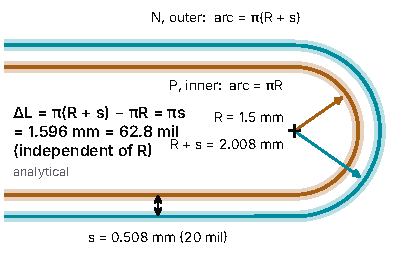
\includegraphics[width=\columnwidth]{fig_bend}
\caption{\textbf{Analytical.} Centrelines of P (inner) and N (outer) around the 180-degree bend of fixture B. The
arc lengths differ by $\pi s$ whatever the radius.}
\label{fig:bend}
\end{figure}

\textbf{The fixture.} One microstrip layer over a return plane (Fig.~\ref{fig:ports}, Table~\ref{tab:params}):
$h = 0.2$\,mm, $\varepsilon_r = 4.3$, $w = 0.25$\,mm, $s = 0.508$\,mm. Every bent variant uses the same U-bend
($R = 1.5$\,mm for P), the same 12\,mm legs and the same launch plane, so only the tuning differs
(Fig.~\ref{fig:families}):
A, a straight pair of the U-bend's mean length; B, the untuned bend; C, two sparse excursions next to the bend;
C far, the same two excursions next to the launch; D, a dense accordion of four; F, one broad trombone; and E, a
pair-level raised-cosine excursion of both traces together, a control whose net turning angle is zero and which
therefore leaves the length difference unchanged. Each single-trace tuning is cut into P on the leg leading into
the bend and turns away from N. Every route length change is intentional and listed in
Table~\ref{tab:metrics}. Clearance between P and N copper is checked by our generator and by KiCad~10's DRC
(\texttt{kicad-cli pcb drc}, 0.15\,mm rule): no clearance or short violation in any variant. KiCad does not check
spacing within one net, so the fold spacing is set by the parameters: \FoldD\,mm edge to edge in D.

\begin{figure*}[t]
\centering
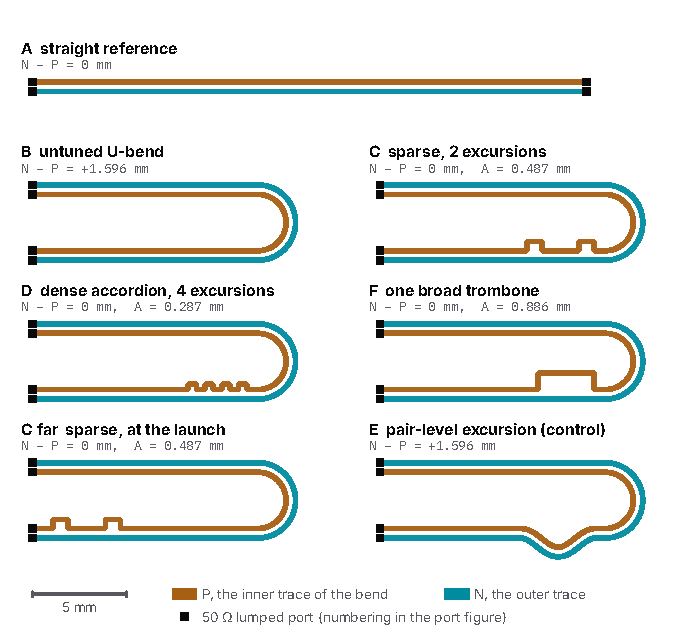
\includegraphics[width=0.93\textwidth]{fig_families}
\caption{The variants, drawn from the copper polygons that go into the EM model, at one scale. Every tuned variant
(C, C far, D, F) has P and N exactly equal in centreline length; $A$ is the solved excursion amplitude.}
\label{fig:families}
\end{figure*}

\begin{table}[t]
\centering
\caption{Parameters. All values are \textbf{proposed} for this study; none is calibrated to a laminate or a
fabricator.}
\label{tab:params}
\scriptsize
\adjustbox{max width=\columnwidth}{\begin{tabular}{@{}llll@{}}\toprule
Parameter & Unit & Value & Range or note \\\midrule
Dielectric height $h$ & mm & 0.2 & fixed \\
Relative permittivity $\varepsilon_r$ & -- & 4.3 & fixed \\
Loss tangent at 5 GHz & -- & 0.02 & fixed, $\propto 1/f$ \\
Copper thickness / $\sigma$ & mm / MS/m & 0.035 / 58 & sheet model \\
Trace width $w$ & mm & 0.25 & fixed \\
Pair pitch $s$ (centre to centre) & mm & 0.508 & fixed, 20 mil \\
Bend radius of P, $R$ & mm & 1.5 & 0.75, 1.5, 3.0 \\
Leg length (launch to bend) & mm & 12.0 & fixed \\
Excursions $N$ & -- & 1, 2, 4 & F, C, D \\
Amplitude $A$ & mm & solved & 0.29--1.08 \\
Excursion top / gap & mm & 0.45--3.0 & per family \\
Corner chamfer & mm & 0.075 & fixed \\
Stripline plane spacing & mm & 0.7 & trace midway \\
Distance to bend $D$ & mm & 0.5 & 0.5 or at launch \\
Serpentine added length & mm & 6.0 & fold gap 1.0, 0.15 \\
Edge (10--90\,\%) & ps & 35--300 & post-processing \\
Bandwidth & GHz & 0--30 & Gaussian pulse \\
Finest cell (coarse/medium/fine) & \textmu m & 60/40/27 & convergence \\
\bottomrule\end{tabular}
}
\end{table}

\begin{figure*}[t]
\centering
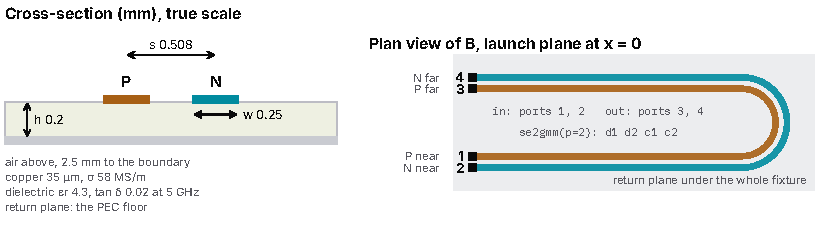
\includegraphics[width=\textwidth]{fig_ports}\\[4pt]
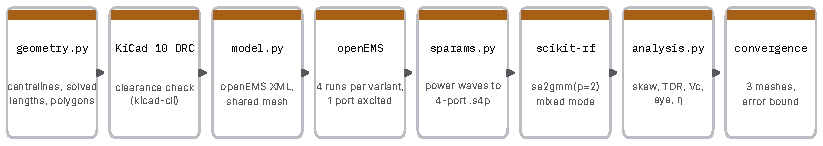
\includegraphics[width=\textwidth]{fig_pipeline}
\caption{Top: cross-section, true scale, and fixture B with its four lumped ports on the launch plane and their
mixed-mode mapping. Bottom: the pipeline. Each run keeps its model, its solver log and a provenance record
(solver version, model hash, wall time, timesteps); each variant keeps its \texttt{.s4p} and its checks.}
\label{fig:ports}\label{fig:pipeline}
\end{figure*}

\section{Numerical model}
\label{sec:model}

\subsection{Stage II: a two-conductor line model}

For the pair, the coupled telegrapher equations are
\begin{equation}
  \frac{\mathrm{d}\mathbf{V}}{\mathrm{d}x} = -(\mathbf{R} + j\omega\mathbf{L})\,\mathbf{I}, \qquad
  \frac{\mathrm{d}\mathbf{I}}{\mathrm{d}x} = -(\mathbf{G} + j\omega\mathbf{C})\,\mathbf{V},
  \label{eq:telegrapher}
\end{equation}
with $2\times2$ per-unit-length matrices whose off-diagonal terms are the coupling~\cite{paul_mtl}. For a
symmetric pair the even and odd modes diagonalise them. Rather than assume a cross-section, we calibrate the modes
on the full-wave straight fixture A: its $\Sdd{}$ (100\,$\Omega$) and $\Scc{}$ (25\,$\Omega$) are each the
two-port of a uniform line, from which the extraction of Eisenstadt and Eo~\cite{eisenstadt1992} gives
$Z_\mathrm{odd} = \ZOdd\,\Omega$ ($Z_\mathrm{diff} = \ZDiff\,\Omega$), $Z_\mathrm{even} = \ZEven\,\Omega$
($Z_\mathrm{comm} = \ZComm\,\Omega$), $\eeff = \EpsOdd$ (odd) and \EpsEven{} (even), with loss and dispersion,
from 0.5 to 10\,GHz. Each variant is then a cascade of chain matrices: coupled sections where the traces run
together, and uncoupled single lines (Hammerstad--Jensen parameters) where P leaves N or where N's excess lies in
the bend, spread over 18 slices. The model knows every length. It does not know corners, coupling between the
folds of a meander, coupling across the U, or the bend as a discontinuity, which is exactly what makes it useful
as a reference: where it disagrees with full wave, length is not the explanation.

\subsection{Stage III: full-wave extraction}

The solver is openEMS~\cite{openems_intro,liebig2013}, an equivalent-circuit FDTD code, version
\texttt{\SolverVersion}. Its Python bindings were not installed on the host, so the model is written directly in
the XML vocabulary those bindings produce, which we had checked against this openEMS version before. The
signal copper is a conducting sheet (35\,$\mu$m, 58\,MS/m) drawn from the generator's polygons; the return plane is
the PEC floor of the domain; the dielectric is a lossy box (Table~\ref{tab:params}; openEMS models the loss as a
fixed conductivity, so $\tan\delta$ falls as $1/f$). The other five faces are first-order Mur absorbing
boundaries~\cite{mur1981}, at least 2\,mm (10$h$) from any copper laterally and 2.5\,mm above it.

Each trace end has a 50\,$\Omega$ lumped port from the plane to the copper, on the launch plane $x = 0$
(Fig.~\ref{fig:ports}). Ports are numbered in scikit-rf's mixed-mode order~\cite{skrf_se2gmm}: 1 = P near,
2 = N near, 3 = P far, 4 = N far. Each variant takes four runs, each exciting one port with the other three
passive~\cite{openems_ports}, with a Gaussian pulse covering 0 to 30\,GHz. From each port's voltage $u_k$ and
current $i_k$ (into the structure), the power waves~\cite{kurokawa1965}
$a_k = (u_k + Z_0 i_k)/(2\sqrt{Z_0})$ and $b_k = (u_k - Z_0 i_k)/(2\sqrt{Z_0})$ give $S_{kj} = b_k/a_j$; the
result is written as a Touchstone \texttt{.s4p} from DC to 30\,GHz in 10\,MHz steps.

The mesh is rectilinear and graded: finest cells over the copper regions (60, 40 and 27\,$\mu$m for the coarse,
medium and fine levels, with every straight trace edge on a grid line), growing by at most 1.3 per cell to
0.15\,mm laterally and 0.3\,mm in the air. All bent variants share one mesh per level, built over the union of
their copper, so discretisation error in the copper they share is common to them. The medium mesh of the bent
fixtures has \CellsMedium\,M cells; the fine one \CellsFine\,M. The arcs and chamfers are staircased.

One behaviour of the solver needed care. The pulse's DC content leaves a static field in the domain whose energy
settles near $-38$\,dB, so no run reaches an energy end criterion; a pulse without DC content does, but it
measures nothing useful below about 2\,GHz. Every run therefore stops at a fixed 2\,ns of simulated time, by which
the port voltages have fallen at least \TruncWorst\,dB below their peak (Table~\ref{tab:checks}); on fixture B
(coarse mesh, port 1 excited) a 7\,ns record changes the low-frequency S-parameters by about $10^{-3}$.

\section{Analysis metrics}
\label{sec:metrics}

\textbf{Mixed mode.} \texttt{se2gmm(p=2)} on the order above gives $d_\mathrm{near}, d_\mathrm{far},
c_\mathrm{near}, c_\mathrm{far}$, so $\Sdd{11}=S_{00}$, $\Sdd{21}=S_{10}$, $\Scd{21}=S_{30}$ (zero-based), with
reference impedances of 100\,$\Omega$ differential and 25\,$\Omega$ common, in scikit-rf~\cite{arsenovic2022}. We
checked this convention against the scikit-rf 2.2.0 source rather than its rendered documentation.

\textbf{Waveforms.} A differential step of 1\,V open circuit (+1\,V and $-1$\,V, each behind 50\,$\Omega$) with a
Gaussian edge of 10--90\,\% rise time $t_r$ drives ports 1 and 2; ports 3 and 4 are 50\,$\Omega$ to the plane
(100\,$\Omega$ differential, 25\,$\Omega$ common). Far-end voltages follow by superposition from the four-port in
the frequency domain and an inverse FFT; nothing is fitted. $V_d = V_P - V_N$, $V_c = (V_P + V_N)/2$.

\textbf{Skew} is $t_{50}(N\ \text{falling}) - t_{50}(P\ \text{rising})$ at the far end, each at half its own final
value; positive means P, the inner trace, arrives first. We report 50\,ps edges unless stated, and 35 to 300\,ps
in Section~\ref{sec:results}. Edges faster than 35\,ps are not evaluated, because the simulated band ends at
30\,GHz.

\textbf{Delay efficiency.}
\begin{equation}
  \eta = \frac{t_\mathrm{skew,ref} - t_\mathrm{skew}}{\Delta L_\mathrm{add}\sqrt{\eeff^\mathrm{single}}/c},
  \label{eq:eta}
\end{equation}
where the reference is the identical untuned fixture (B, or the straight serpentine reference), $\Delta
L_\mathrm{add}$ is the centreline the tuning adds to P, and $\eeff^\mathrm{single} = \EpsSingle$
(\PsPerMm\,ps/mm) is the velocity a designer's length-to-delay conversion would use. $\eta = 1$ means the delay
is what the length predicts. On the same basis the untuned bend has $\eta = \BendEta$.

\textbf{Other metrics}, each over 0.1--20\,GHz unless stated: worst $|\Sdd{11}|$; RMS $|\Scd{21}|$; differential
TDR impedance from the step response of $\Sdd{11}$ with a 35\,ps edge; the frequency-resolved skew of
Eq.~\eqref{eq:fdskew}; a PRBS7 eye at 10\,Gb/s (50\,ps edges) and 16\,Gb/s (35\,ps edges), with height at the
best phase and width where the eye is open by more than 10\,\% of the swing; and the board area of the tuning,
its length times its amplitude. No interface specification is assumed: wherever a pass or fail would need one, the
target is illustrative and is to be selected for the intended interface.

\begin{table*}[t]
\centering
\caption{Metrics, medium mesh, 50\,ps edge. $\Delta L_\mathrm{add}$ is the centreline the tuning adds to P;
$\eta$ is Eq.~\eqref{eq:eta}; MTL is the line model's skew; $|\Sdd{11}|$ and $|\Scd{21}|$ over 0.1--20\,GHz;
$Z_\mathrm{diff}$ from TDR. Skew bounds: each variant's own GCI where it was solved on three meshes, else that of the converged variant
whose smallest features it shares (Section~\ref{sec:verification}).}
\label{tab:metrics}
\footnotesize
\adjustbox{max width=\textwidth}{% metric table
\begin{tabular}{@{}lrrrrrrrrr@{}}\toprule
Variant & $\Delta L_\mathrm{add}$ & Skew & $\eta$ & MTL & $V_c$ p-p & $|S_{dd11}|$ & $|S_{cd21}|$ & $Z_\mathrm{diff}$ & Area \\
 & (mm) & (ps) & & (ps) & (\%) & max (dB) & RMS (dB) & max ($\Omega$) & (mm$^2$) \\\midrule
A straight & -- & 0.00 $\pm$ 0.05 & -- & 0.00 & 0.00 & -23.4 & -- & 106.0 & 0.00 \\
B untuned & -- & 9.27 $\pm$ 0.05 & -- & 8.83 & 4.87 & -20.7 & -10.2 & 107.1 & 0.00 \\
E pair exc. & -- & 9.39 $\pm$ 0.05 & -- & 8.83 & 4.92 & -21.4 & -10.1 & 108.1 & 4.00 \\
C sparse & 1.596 & 3.59 $\pm$ 0.31 & 0.60 & 0.31 & 1.83 & -21.6 & -18.0 & 106.9 & 1.83 \\
C far & 1.596 & 4.36 $\pm$ 0.31 & 0.52 & 0.96 & 2.19 & -19.6 & -15.4 & 106.9 & 1.83 \\
D dense & 1.596 & 5.16 $\pm$ 0.43 & 0.44 & 0.27 & 2.67 & -19.8 & -14.9 & 106.9 & 0.95 \\
F trombone & 1.596 & 2.29 $\pm$ 0.31 & 0.74 & 0.23 & 1.16 & -16.8 & -22.0 & 114.4 & 2.79 \\
C, EM-sized & 2.213 & 0.56 $\pm$ 0.31 & 0.66 & -2.98 & 0.52 & -21.7 & -25.2 & 106.7 & 2.40 \\
D, EM-sized & 2.484 & 1.90 $\pm$ 0.43 & 0.50 & -4.50 & 0.98 & -19.9 & -22.6 & 106.7 & 1.31 \\
F, EM-sized & 1.991 & 0.15 $\pm$ 0.31 & 0.77 & -1.89 & 0.40 & -16.7 & -27.8 & 115.0 & 3.41 \\
\bottomrule\end{tabular}
}
\end{table*}

\begin{figure*}[t]
\centering
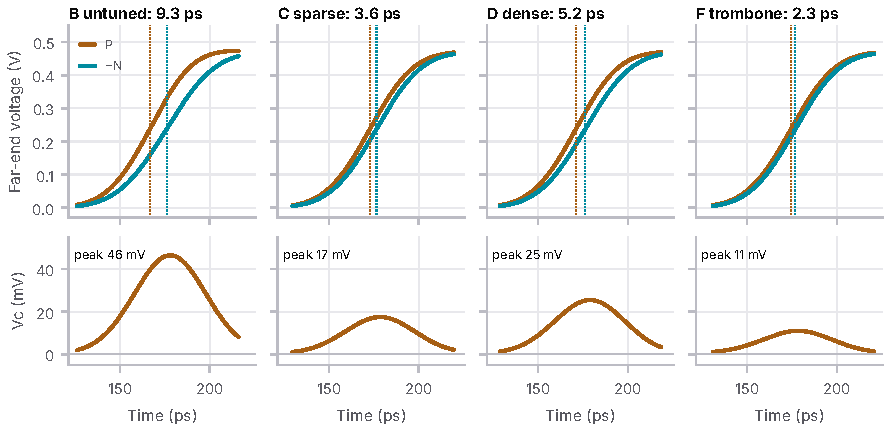
\includegraphics[width=\textwidth]{fig_waveforms}
\caption{Far-end P and $-$N for a differential step (50\,ps edge), and the common-mode voltage. Dotted lines mark
each 50\,\% crossing.}
\label{fig:waveforms}
\end{figure*}

\section{Verification of the numerics}
\label{sec:verification}

Table~\ref{tab:checks} lists the checks for every variant. Reciprocity holds to $|S_{ij}-S_{ji}| \le$
\RecipMax{} (the straight fixture, symmetric by construction, to \RecipA). Every four-port is passive: the
largest singular value of $S$ over the band is \PassB{} for B and no more than \PassMax{} for any variant. Every
record ends with its port voltages at least \TruncWorst\,dB below their peak.

\textbf{Convergence.} B, C, D and the serpentine set were solved on three meshes, and D on a fourth
(Table~\ref{tab:conv}, Fig.~\ref{fig:conv}). We report Roache's grid convergence index~\cite{roache1994}
over the three finest meshes, with safety factor 1.25 and an observed order capped at the scheme's formal order
of 2; where those meshes do not converge monotonically we use three times their spread. B converges monotonically, to within \GciB\,ps on the finest mesh. D's 75\,$\mu$m chamfers span barely one cell
on the coarse mesh, and its coarse value is the outlier; over the three finest meshes it converges monotonically,
to \ExtD\,ps. The tight serpentine's 0.15\,mm folds still oscillate across meshes. The comparison tables quote the
medium mesh throughout, so each medium value carries its own bound: 1.25 times its distance from the extrapolated
value, or three times the spread where the meshes oscillate (Table~\ref{tab:conv}): $\pm$\BoundMedB\,ps for B,
$\pm$\BoundMedC\,ps for C and $\pm$\BoundMedD\,ps for D, whose medium value runs high by about that much. A
variant solved on the medium mesh only carries the bound of the converged variant whose smallest features it
shares: C's for C far, F and the EM-sized C and F; D's for the EM-sized D; B's for E and the other bend radii.
Because a wide bound can hide a
trend or invent one, we also judge every conclusion mesh by mesh: Table~\ref{tab:etalevels} gives $\eta$ on
each mesh, each against its untuned reference on the same mesh.

\begin{table}[t]
\centering
\caption{Numerical checks (medium mesh). Truncation is how far every port voltage had fallen, relative to its
peak, over the last 5\,\% of the record.}
\label{tab:checks}
\scriptsize
\adjustbox{max width=\columnwidth}{\begin{tabular}{@{}lrrr@{}}\toprule
Variant & Reciprocity & Passivity & Truncation \\
 & $\max|S_{ij}-S_{ji}|$ & $\max\sigma(S)$ & (dB) \\\midrule
A straight & $3.3\times10^{-7}$ & 0.989 & -110 \\
B untuned & $2.4\times10^{-3}$ & 0.989 & -110 \\
C sparse & $4.5\times10^{-3}$ & 0.988 & -110 \\
C far & $2.8\times10^{-3}$ & 0.988 & -109 \\
D dense & $3.4\times10^{-3}$ & 0.988 & -110 \\
E pair exc. & $2.9\times10^{-3}$ & 0.988 & -110 \\
F trombone & $2.8\times10^{-3}$ & 0.988 & -110 \\
C, EM-sized & $3.7\times10^{-3}$ & 0.988 & -110 \\
D, EM-sized & $3.0\times10^{-3}$ & 0.988 & -110 \\
F, EM-sized & $2.0\times10^{-3}$ & 0.988 & -110 \\
Serp. ref. & $6.0\times10^{-5}$ & 0.989 & -110 \\
Serp. 1.0 mm & $1.8\times10^{-3}$ & 0.988 & -109 \\
Serp. 0.15 mm & $2.1\times10^{-3}$ & 0.988 & -109 \\
B, R 0.75 & $3.5\times10^{-3}$ & 0.990 & -110 \\
B, R 3.0 & $2.4\times10^{-3}$ & 0.987 & -108 \\
B stripline & $1.8\times10^{-3}$ & 0.989 & -109 \\
C stripline & $1.4\times10^{-3}$ & 0.988 & -109 \\
D stripline & $1.8\times10^{-3}$ & 0.988 & -110 \\
F stripline & $2.2\times10^{-3}$ & 0.988 & -109 \\
Serp. ref. SL & $2.9\times10^{-5}$ & 0.988 & -99 \\
Serp. 1.0 mm SL & $1.5\times10^{-3}$ & 0.987 & -98 \\
Serp. 0.15 mm SL & $1.5\times10^{-3}$ & 0.987 & -98 \\
\bottomrule\end{tabular}
}
\end{table}

\begin{table}[t]
\centering
\caption{Mesh convergence of the skew (50\,ps edge).}
\label{tab:conv}
\scriptsize
\adjustbox{max width=\columnwidth}{\begin{tabular}{@{}lrrrrrrl@{}}\toprule
Variant & 60\,\textmu m & 40\,\textmu m & 27\,\textmu m & 18\,\textmu m & GCI & 40\,\textmu m & Convergence \\
 & (ps) & (ps) & (ps) & (ps) & finest & bound & \\\midrule
B untuned & 9.54 & 9.27 & 9.25 & -- & $\pm$0.02 & $\pm$0.05 & monotonic \\
C sparse & 3.69 & 3.59 & 3.61 & -- & $\pm$0.31 & $\pm$0.31 & oscillatory \\
D dense & 4.45 & 5.16 & 4.88 & 4.84 & $\pm$0.03 & $\pm$0.43 & monotonic \\
Serp. ref. & 0.03 & 0.03 & 0.03 & -- & $\pm$0.00 & $\pm$0.00 & monotonic \\
Serp. 1.0 mm & -32.41 & -29.99 & -29.69 & -- & $\pm$0.31 & $\pm$0.68 & monotonic \\
Serp. 0.15 mm & -23.63 & -24.12 & -22.98 & -- & $\pm$3.40 & $\pm$3.40 & oscillatory \\
\bottomrule\end{tabular}
}
\end{table}

\begin{table}[t]
\centering
\caption{Delay efficiency $\eta$ (Eq.~\ref{eq:eta}) on each mesh, against the untuned reference on the same
mesh.}
\label{tab:etalevels}
\scriptsize
\adjustbox{max width=\columnwidth}{\begin{tabular}{@{}lrrrr@{}}\toprule
$\eta$ on each mesh & 60\,\textmu m & 40\,\textmu m & 27\,\textmu m & 18\,\textmu m \\\midrule
C sparse & 0.62 & 0.60 & 0.60 & -- \\
D dense & 0.54 & 0.44 & 0.46 & 0.47 \\
Serp. 1.0 mm & 0.91 & 0.84 & 0.84 & -- \\
Serp. 0.15 mm & 0.67 & 0.68 & 0.65 & -- \\
\bottomrule\end{tabular}
}
\end{table}

\begin{figure}[t]
\centering
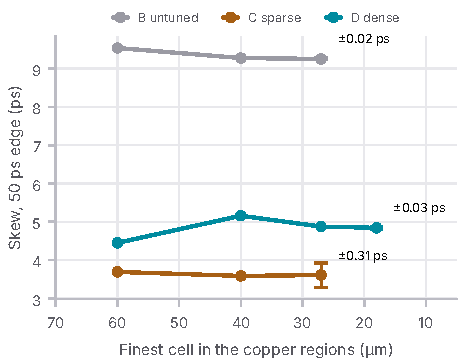
\includegraphics[width=\columnwidth]{fig_convergence}
\caption{Skew against the finest cell size. The bar on each variant's finest point is its GCI bound.}
\label{fig:conv}
\end{figure}

\section{Results}
\label{sec:results}

All values in this section are simulated; Table~\ref{tab:metrics} collects them.

\subsection{The untuned bend}

B shows \SkewB\,ps of skew at 50\,ps edges, against \SkewSingle\,ps from Eq.~\eqref{eq:dt} with the single-line
$\eeff$. Geometry predicts the bend well. The skew does depend on the edge: \SkewBRdf\,ps at 35\,ps and
\SkewBRdaa\,ps at 300\,ps (Fig.~\ref{fig:rise}), moving from near the odd-mode prediction (\SkewOdd\,ps) toward
the even-mode one (\SkewEven\,ps) as the edge slows. The bend radius matters a little where Eq.~\eqref{eq:dl} says
it should not: \SkewBRsmall\,ps at $R = 0.75$\,mm, \SkewB\,ps at 1.5\,mm and \SkewBRlarge\,ps at 3\,mm
(Fig.~\ref{fig:radius}). The pair-level excursion E leaves the skew where B has it (\SkewE\,ps) and adds
\DelayAddE\,ps of pair delay; as designed, it is not an intra-pair fix.

\subsection{Equal length is not equal delay}

Fig.~\ref{fig:skew} is the central result. Every single-trace tuning makes P and N exactly equal in centreline
length, and every one leaves skew: \SkewF\,ps for the broad trombone F, \SkewC\,ps for the two sparse excursions
C ($\pm$\UncC{} on each), and \SkewD\,ps for the dense accordion D ($\pm$\UncD; \ExtD\,ps converged). In efficiency terms
(Eq.~\eqref{eq:eta}), $\eta = \EtaF$, \EtaC{} and \EtaD{}: one, two and four excursions. The transmission-line
model, given the same lengths, predicts \MtlF, \MtlC{} and \MtlD\,ps. The waveforms (Fig.~\ref{fig:waveforms})
show the same thing at the receiver: P still leads N, and the common-mode pulse falls from
\(\VcB\)\,\% of the step for B to \VcF--\VcD\,\%, not to zero.

\begin{figure}[t]
\centering
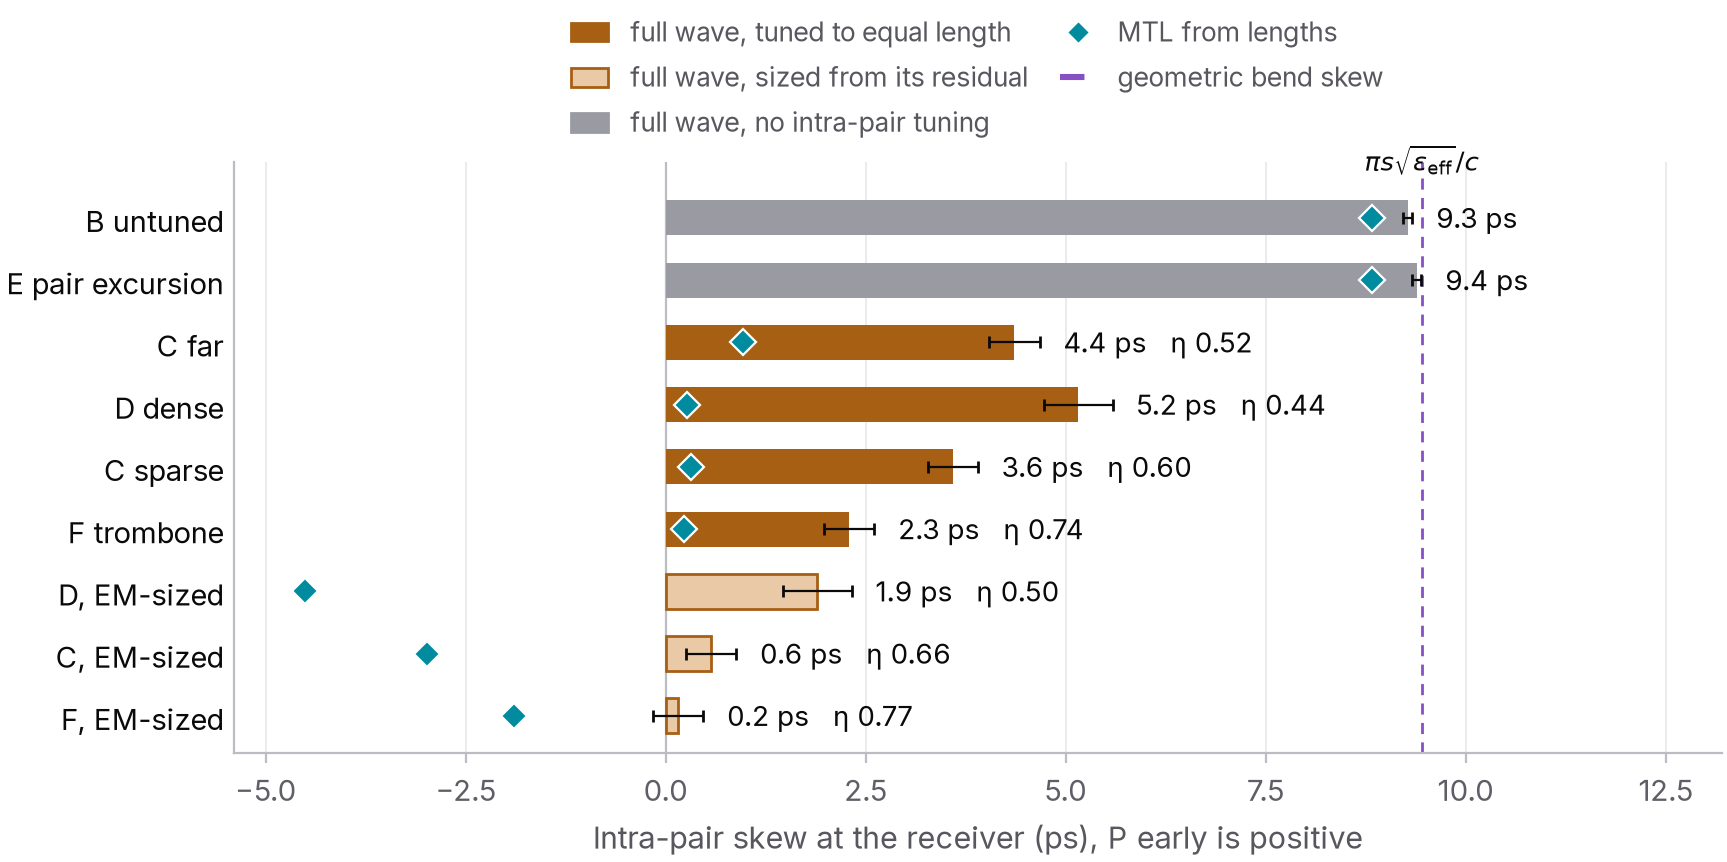
\includegraphics[width=\columnwidth]{fig_skew}
\caption{Skew at the receiver, 50\,ps edge. Copper: tuned to exactly equal length. Grey: no intra-pair tuning.
Diamonds: the transmission-line model with the same lengths. Bars: numerical uncertainty.}
\label{fig:skew}
\end{figure}

\begin{figure*}[t]
\centering
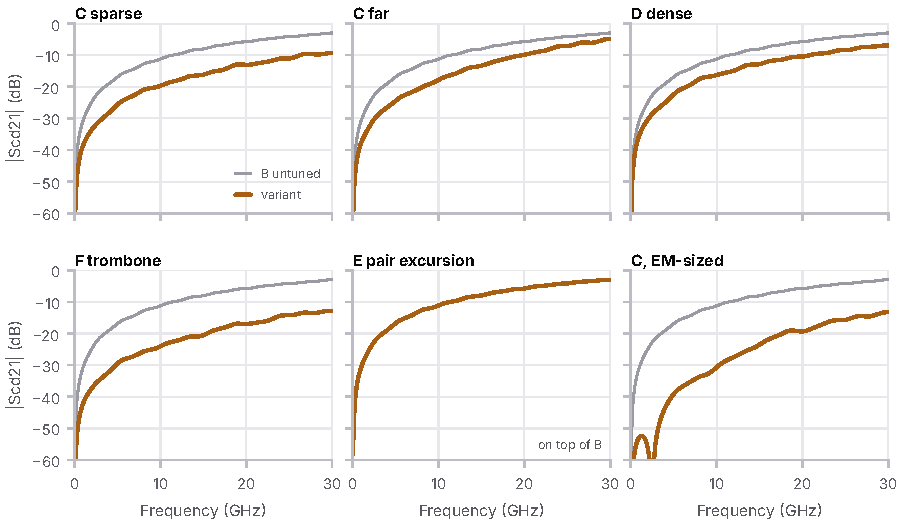
\includegraphics[width=\textwidth]{fig_scd21}
\caption{$|\Scd{21}|$ of each variant (copper) against the untuned bend B (grey).}
\label{fig:scd21}
\end{figure*}

\subsection{Where the delay goes}

The gap is consistent with two effects that the line model leaves out. The serpentine experiment isolates them: a
straight pair with 6\,mm added to P in three excursions, once with folds 1.0\,mm apart (5$h$) and once 0.15\,mm
apart, the clearance rule. The two have the same corners and the same added length. With loose folds
$\eta = \EtaSloose$ (\EtaMinSloose--\EtaMaxSloose{} across the meshes); with tight folds $\eta = \EtaStight$
(\EtaMinStight--\EtaMaxStight), \FoldPenMin{} to \FoldPenMax{} points lower on every mesh
(Fig.~\ref{fig:eta}, Table~\ref{tab:etalevels}). Coupling between the folds is the
difference between them; the loose serpentine's own shortfall, which the line model also misses, we attribute to its
twelve corners. In the bend corrections the shortfall per excursion, full wave less the line model, is
\PerExcMin{} to \PerExcMax\,ps for this trace width, and it does not scale with the length added, so a correction made of more, smaller excursions
under-delivers more. The dense accordion D has the most corners and the closest folds, and the lowest $\eta$.

\begin{figure}[t]
\centering
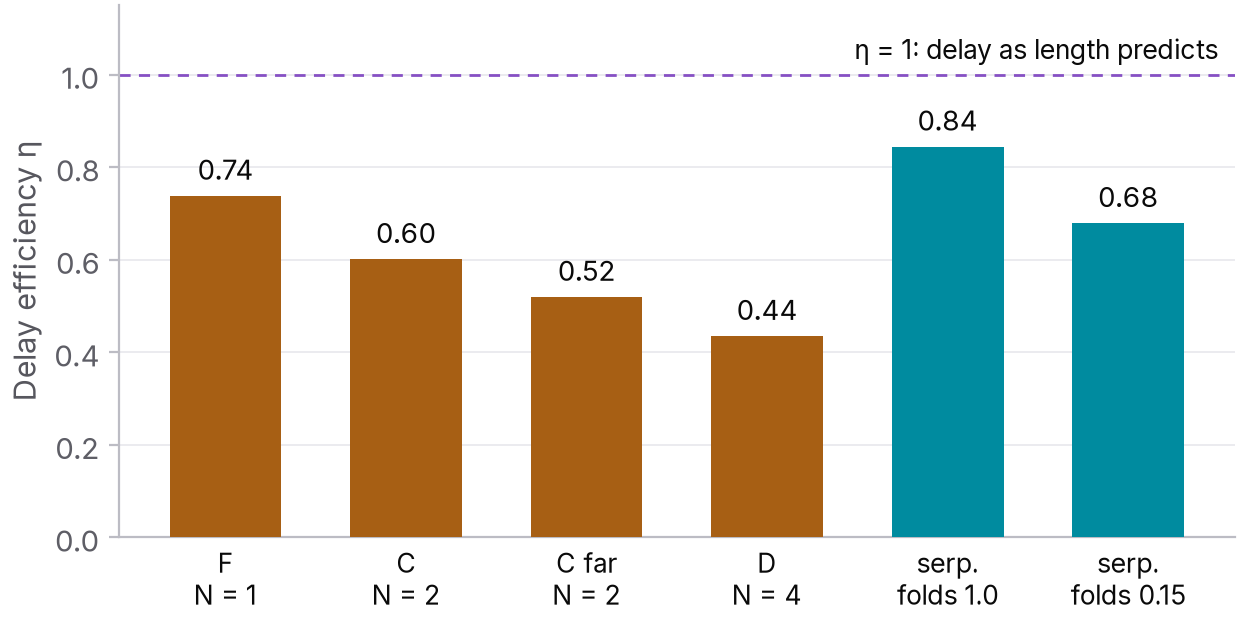
\includegraphics[width=\columnwidth]{fig_eta}
\caption{Delay efficiency $\eta$ (Eq.~\ref{eq:eta}) of the bend corrections (copper, $N$ excursions) and of the
6\,mm serpentines (teal) with loose and tight folds.}
\label{fig:eta}
\end{figure}

\begin{figure*}[t]
\centering
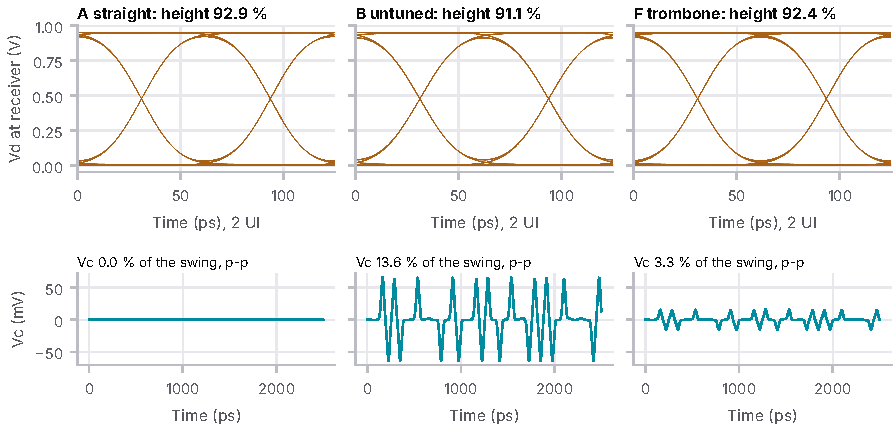
\includegraphics[width=\textwidth]{fig_eye}
\caption{16\,Gb/s PRBS7 eyes (35\,ps edges) and the common-mode voltage at the receiver.}
\label{fig:eye}
\end{figure*}

\subsection{Stripline}

Everything above is microstrip, where the odd and even modes travel at different velocities. To see whether that
matters, we solved B, C, D, F and the serpentine set again in stripline: the same copper midway between two
planes 0.7\,mm apart, with the ports to the lower plane. Stripline is homogeneous, so its nominal velocity is
$c/\sqrt{\varepsilon_r}$ (\PsPerMmSl\,ps/mm) and Eq.~\eqref{eq:eta} uses that. Geometry predicts the bend to
\BendErrPctSl\,\% (\SkewBsl\,ps against \SkewGeoSl\,ps). The length-matched tunings remove \RemovedPctFsl,
\RemovedPctCsl{} and \RemovedPctDsl\,\% of it for F, C and D, against \RemovedPctF, \RemovedPctC{} and
\RemovedPctD\,\% in microstrip, and the serpentines give $\eta = \EtaSloosesl$ and \EtaStightsl, a fold
penalty of \FoldPenaltySl{} points against \FoldPenalty{} in microstrip (Fig.~\ref{fig:stripline}). We had
expected less: in a homogeneous medium the far-end coupling between parallel lines vanishes. But the folds of a
meander carry current in opposite directions, so what couples them acts backward along the route, and that
coupling is present in both media. These stripline runs are on the medium mesh only.

\begin{figure}[t]
\centering
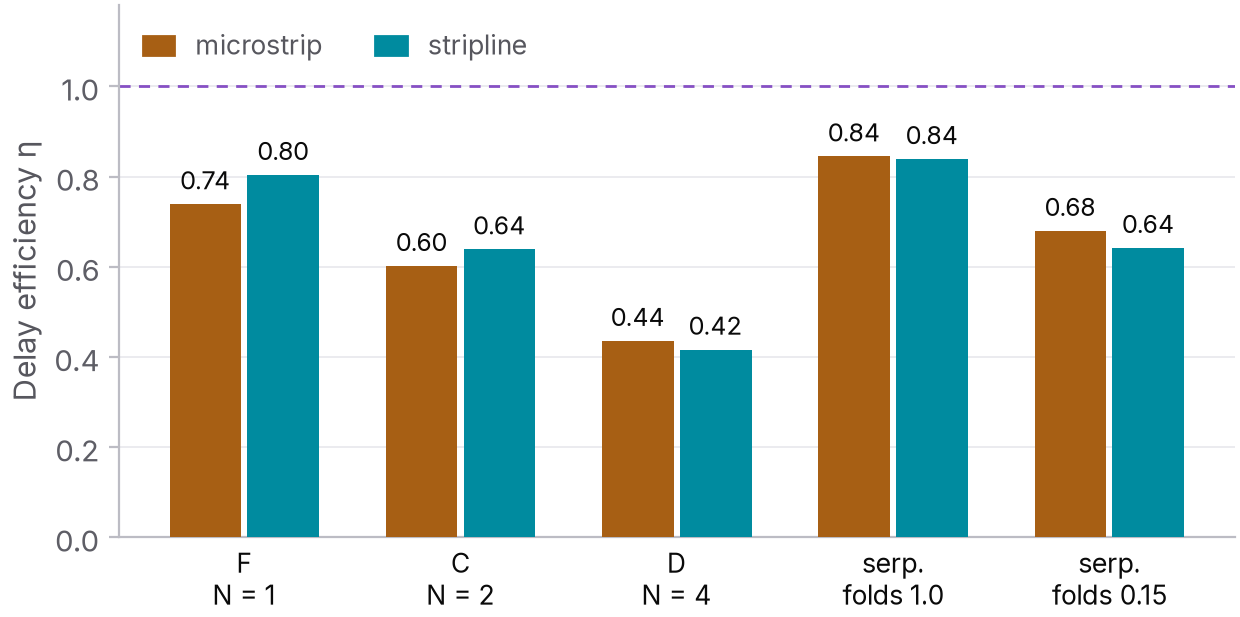
\includegraphics[width=\columnwidth]{fig_stripline}
\caption{Delay efficiency of the same copper in microstrip and in stripline, each against its own nominal
velocity.}
\label{fig:stripline}
\end{figure}

\subsection{Placement}

C far is the same tuning as C, next to the launch instead of the bend. Its arrival skew is close
(\SkewCfar{} against \SkewC\,ps), but its mode conversion is not. Between the tuning and the bend the pair
carries a skew in the other direction, and the two conversions drift apart in phase with frequency: the
frequency-resolved skew of C far climbs from \FdCfarGf\,ps at 5\,GHz to \FdCfarGcf\,ps at 25\,GHz, while C stays
near \FdCGf\,ps (Fig.~\ref{fig:fdskew}). Its peak $|\Scd{21}|$ to 20\,GHz is \ScdMaxCfar\,dB against
\ScdMaxC\,dB for C. Compensation belongs next to the mismatch.

\begin{figure}[t]
\centering
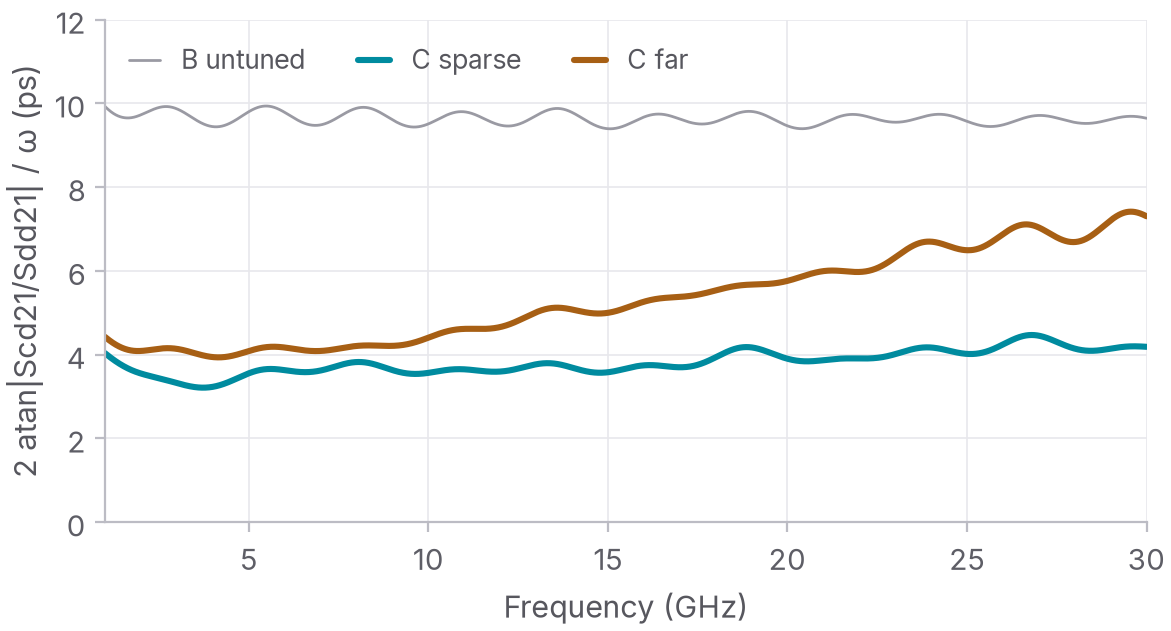
\includegraphics[width=\columnwidth]{fig_fd_skew}
\caption{Frequency-resolved skew from Eq.~\eqref{eq:fdskew}. Compensation far from the bend (C far) holds at low
frequency and fails as frequency rises.}
\label{fig:fdskew}
\end{figure}

\subsection{Reflection, impedance and mode conversion}

Where a trace leaves its partner, the differential impedance rises. The broad trombone F, whose P moves \AmpF\,mm further from N for 3\,mm, lifts $Z_\mathrm{diff}$ to \ZmaxF\,$\Omega$ against \ZmaxB\,$\Omega$ for the untuned bend
(Fig.~\ref{fig:tdr}), and has the worst return loss of the set (\SddMaxF\,dB against \SddMaxB\,dB,
Fig.~\ref{fig:sdd}). So the variant with the least residual skew pays for it in reflection. The dense accordion
barely moves $Z_\mathrm{diff}$. Mode conversion follows the residual skew (Fig.~\ref{fig:scd21}); E's is on top
of B's.

\begin{figure}[t]
\centering
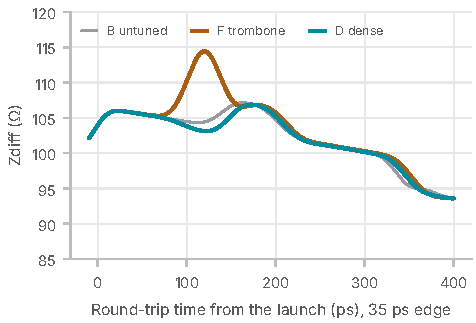
\includegraphics[width=\columnwidth]{fig_tdr}
\caption{Differential TDR (35\,ps edge). F's uncoupled stretch shows as the peak near 120\,ps.}
\label{fig:tdr}
\end{figure}

\begin{figure}[t]
\centering
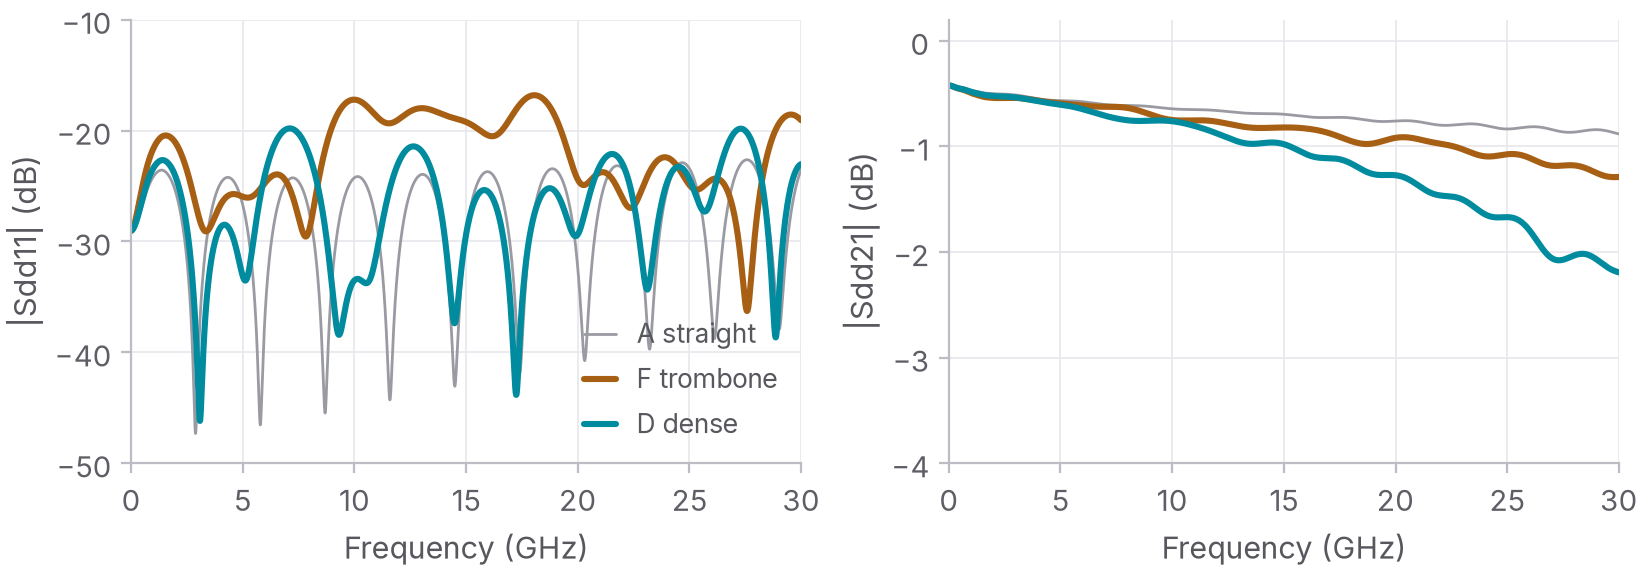
\includegraphics[width=\columnwidth]{fig_sdd}
\caption{Differential return and insertion loss of the straight reference A, the trombone F and the dense
accordion D.}
\label{fig:sdd}
\end{figure}

\begin{figure}[t]
\centering
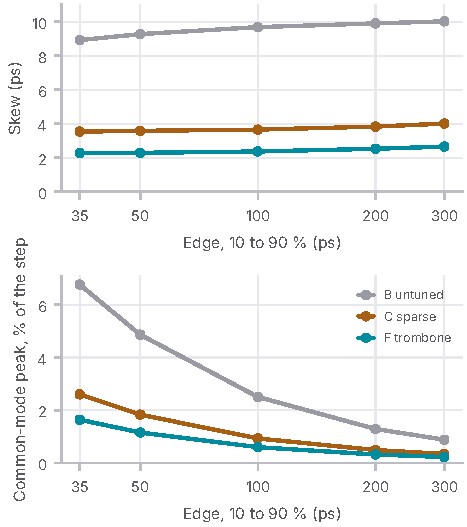
\includegraphics[width=\columnwidth]{fig_rise}
\caption{Skew and peak common-mode voltage against the edge rate.}
\label{fig:rise}
\end{figure}

\subsection{What the skew does to a signal}

At 16\,Gb/s with 35\,ps edges, the untuned bend closes the differential eye from \EyeHA\,\% to \EyeHB\,\% of the
swing and leaves its width at \EyeWB\,UI (Fig.~\ref{fig:eye}). The larger effect is common mode: \EyeVcB\,\% of
the swing peak to peak at the receiver, against \EyeVcF\,\% for F. For a receiver with good common-mode rejection
the skew of a single bend is a common-mode problem more than a timing one. Whether that common mode radiates
depends on the structure beyond the pair, which this study does not model.

\begin{figure}[t]
\centering
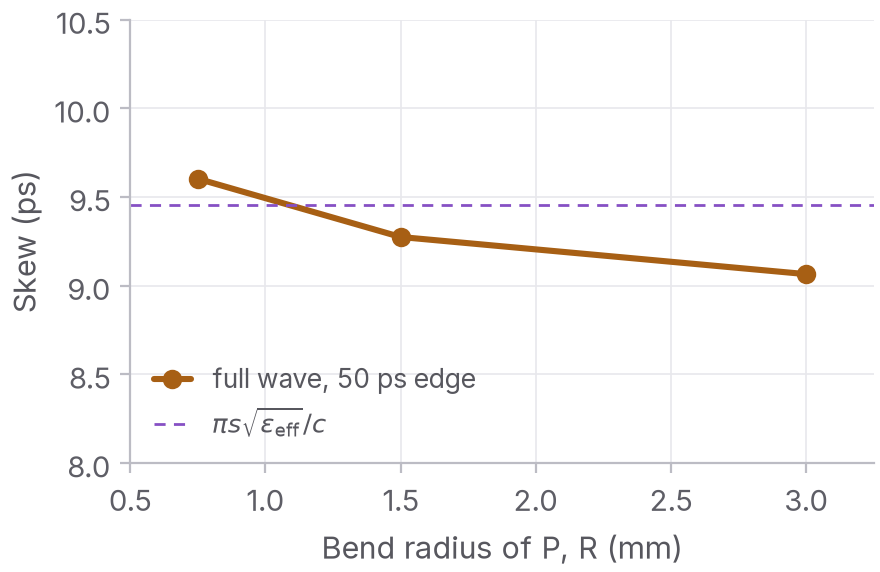
\includegraphics[width=\columnwidth]{fig_radius}
\caption{Skew of the untuned bend against its radius.}
\label{fig:radius}
\end{figure}

\section{Optimization}
\label{sec:optimization}

\textbf{EM-informed sizing.} If each excursion loses a fixed amount of delay to its corners and folds, more
amplitude on the same excursions should recover it. We lengthened C, D and F by their own medium-mesh residual,
converted to length at the bend's rate ($\Delta L_\mathrm{add} = \pi s\,(1 + t_\mathrm{skew}/t_\mathrm{skew,B})$),
so that by CAD measure P is now longer than N, by \AddedCcal, \AddedDcal{} and \AddedFcal\,mm in total added.
By length alone these variants now overshoot: the line model, which sees only lengths, predicts \MtlFcal,
\MtlCcal{} and \MtlDcal\,ps. Full wave gives \SkewFcal\,ps for F and \SkewCcal\,ps for C, within or close to
their numerical bound, but \SkewDcal\,ps for D. The fixed-shortfall model is the reason: the extra millimetres delivered
\MargPctF\,\% of their expected delay in F and \MargPctC\,\% in C, but only \MargPctD\,\% in D, whose
lengthened verticals couple more strongly to one another. A broad or sparse tuning is calibrated by one field
solution or one set of coupons per stackup, and a tuner could carry the per-excursion correction; a dense
accordion needs iteration, which is one more reason to avoid it.

\textbf{Pareto comparison.} Over the bent candidates we minimise four objectives, each defined above: $|t_\mathrm{skew}|$
(50\,ps edge), RMS $|\Scd{21}|$, worst $|\Sdd{11}|$, and tuning area. No weighted score is used. The
non-dominated set is \{\ParetoAll\}. Fig.~\ref{fig:pareto} shows two projections: against area, the dense
accordion is cheap and weak; against return loss, the trombone trades reflection for skew.

\begin{figure*}[t]
\centering
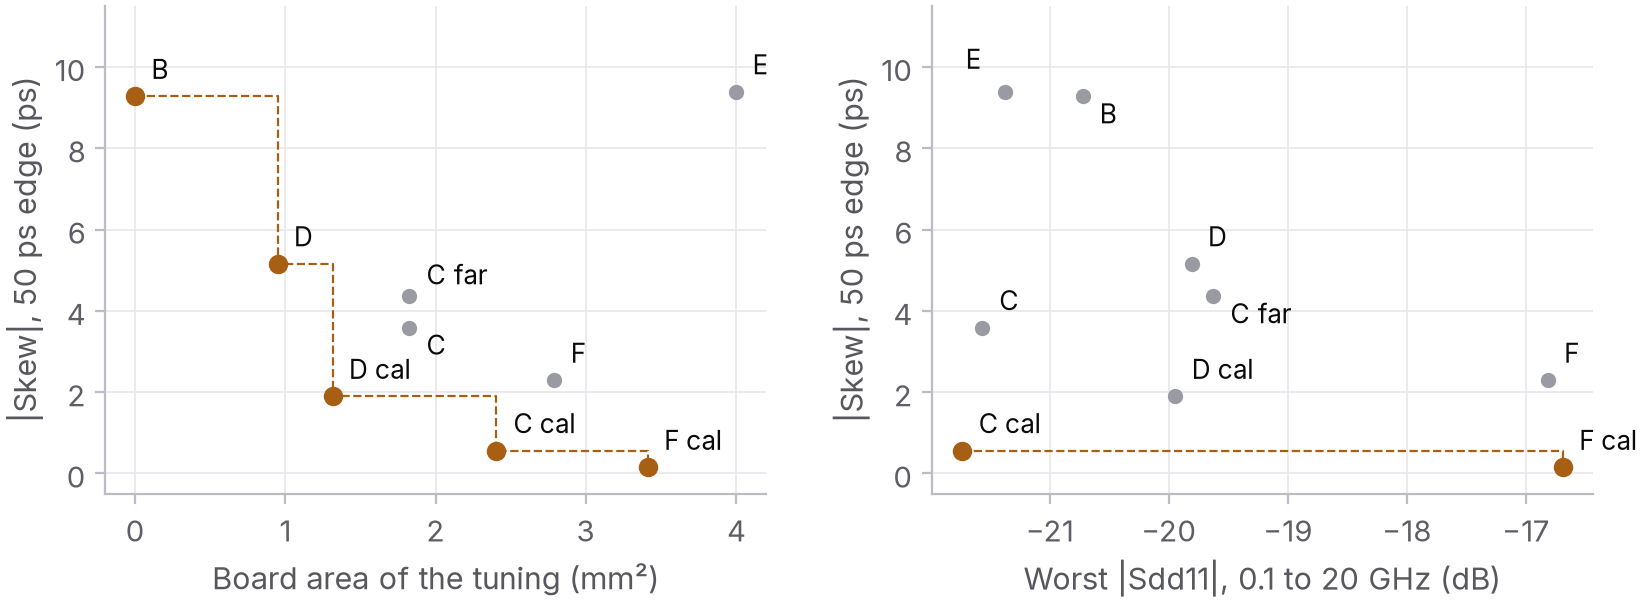
\includegraphics[width=\textwidth]{fig_pareto}
\caption{Two projections of the four-objective comparison. Copper points are non-dominated in that projection;
the dashed line joins them.}
\label{fig:pareto}
\end{figure*}

\section{Physical validation plan}
\label{sec:validation}

Not executed. A coupon panel with one coupon per variant (A--F, the EM-sized variants and the serpentines), each
in three copies, on one laminate and stackup, with identical launches: edge-mount connectors or GSSG probe pads
with ground vias, and a 2x-thru of the launch alone on the same panel for fixture de-embedding as in IEEE
Std~370~\cite{ieee370}. Measure four-port S-parameters to 30\,GHz on a calibrated VNA, de-embed to the launch
plane, and microsection one coupon per panel to measure $w$, $s$, $h$ and the copper. Extract $\eeff$ of the odd
and even modes from coupon A and rerun the EM with the measured dimensions before comparing. The comparison is
skew, $\eta$ (Eq.~\ref{eq:eta}, against B on the same panel), $|\Sdd{11}|$, $|\Scd{21}|$ and TDR, with error bars
from the spread of the three copies, the VNA's stated uncertainty and the GCI here. The predictions to test are
that equal-length tuning leaves \SkewF{} to \SkewD\,ps at this pitch, that the shortfall grows with the excursion
count, and that the same holds on a stripline panel.
Near- or far-field scanning would be needed only if emission is the claim, which it is not here.

\section{Recommendations}
\label{sec:recommendations}

For edge-coupled pairs at this pitch and coupling, in microstrip and in stripline, and with the caveat that the
numbers are simulated:
\begin{itemize}\itemsep 1pt
\item Expect geometry to predict a bend's skew well (here within \BendErrPct\,\%), and expect it to over-predict what a
length-matched tuning removes. Budget a residual, or size the tuning from a field solution or a coupon.
\item Prefer few excursions. Each one costs delay in its corners regardless of its amplitude; a single excursion
removed \RemovedPctF\,\% of the skew, four removed \RemovedPctD\,\%.
\item Keep folds apart. Here folds at the clearance rule lost \FoldPenMin--\FoldPenMax{} points of efficiency
against folds
5$h$ apart.
\item Tune next to the mismatch. The same correction at the launch matches arrival time but not phase at high
frequency.
\item Watch the impedance of a broad excursion: the uncoupled stretch lifts $Z_\mathrm{diff}$, here to
\ZmaxF\,$\Omega$. Keep its amplitude small relative to the pitch or keep it short.
\item A pair-level excursion does not fix intra-pair skew.
\item None of this is special to microstrip. In stripline the bend's skew matched geometry to \BendErrPctSl\,\%,
the length-matched tunings removed a similar share, and tight folds cost \FoldPenaltySl{} points. The edge rate and the interface decide whether a few
picoseconds matter; at 16\,Gb/s here they matter more as common mode than as eye closure.
\end{itemize}

\section{Reproducibility}
\label{sec:repro}

The repository holds \texttt{parameters.yaml}; \texttt{scripts/} with the geometry generator (and its KiCad
export and DRC), the openEMS model writer, the run orchestrator with provenance, the S-parameter extraction, the
line model, the analysis, the convergence study and the figure and table generators; and \texttt{figures/}. Every
number in this report is a macro generated from \texttt{build/results/results.json}. Runs were made on one Linux
host, \RunCount{} runs in all, \RunHours\,h of wall time in total on single-threaded solver processes. The
\texttt{README.md} lists the commands; regenerating every figure and table from the stored S-parameters takes a
few minutes.

\section{Limitations}
\label{sec:limitations}

One width and one pitch, in one microstrip and one stripline stackup. The stripline ports run to the lower
plane only, and its plane spacing came from a closed-form estimate; its $Z_\mathrm{diff}$ is about
\ZmaxBsl\,$\Omega$ by TDR, so its absolute return loss is worse than microstrip's, which does not affect the
skew comparisons. The return plane is a perfect conductor and the copper a
conducting sheet, so conductor loss is approximate and roughness is absent. The dielectric loss model has
$\tan\delta \propto 1/f$. Lumped ports at the launch are not a connector or a probe; their reflection is common to
every variant and cancels in the comparisons, but not in absolute return loss. The staircased mesh resolves the
smallest features (the 75\,$\mu$m chamfers) with two to three cells at the medium level; the convergence study
bounds the effect for B, C, D and the serpentines only, and the stripline set was solved on one mesh. Edges faster than 35\,ps and frequencies above 30\,GHz are outside the
simulated band. Common-mode voltage and $\Scd{21}$ are not emissions. Nothing was measured.

\section{Conclusions}

At a 20\,mil pitch a U-bend's skew is what geometry says, about 9\,ps here. Matching the lengths does not remove
it: a length-matched serpentine removed between \RemovedPctD{} and \RemovedPctF\,\% of the skew in full-wave
simulation, and the
remainder grew with the number of excursions and the closeness of the folds. A line model with the same lengths
missed nearly all of it, and the same copper in stripline behaved the same way. One field-solver iteration sized
the broad and sparse tunings to within \SkewFcal{} and \SkewCcal\,ps; the dense accordion needed more. The fix is not more length matching; it is to size the tuning by its electrical effect,
keep it next to the mismatch, and use few, well-separated excursions.

\small
\raggedright
\bibliographystyle{IEEEtran}
\bibliography{references}

\end{document}
